\documentclass[11pt,a4paper]{article}
\usepackage[margin=2.5cm]{geometry}
%\usepackage[a-1b]{pdfx}
\usepackage{microtype}
\usepackage{mathpazo} % nice fonts
\usepackage{amsmath, amssymb, stmaryrd, latexsym, mathtools}
\usepackage{extarrows}
\usepackage{slashed}
\usepackage{natbib}
\usepackage{todonotes}
\usepackage{url}
\usepackage[capitalise,noabbrev,nameinlink]{cleveref}
\usepackage[unicode=true,pdftex,pdfa]{hyperref}
\hypersetup{
  pdftitle={Design Specification for Delegation and Incentives in Cardano},
  pdfauthor={Philipp Kant, Lars Brünjes, Duncan Coutts},
  breaklinks=true,
  bookmarks=true,
  colorlinks=true,
  linkcolor={black},
  citecolor={black},
  urlcolor={blue},
  linkbordercolor={white},
  citebordercolor={white},
  urlbordercolor={white}
}
\usepackage{float}
\floatstyle{boxed}
\restylefloat{figure}

\DeclareMathOperator{\dom}{dom}
\DeclareMathOperator{\range}{range}

\begin{document}

\title{Design Specification for Delegation and Incentives in Cardano \\
       {\small (Version 0.8)} \\
       {\large \sc An IOHK technical report}}

\author{Philipp Kant   \\ {\small \texttt{philipp.kant@iohk.io}} \\
   \and Lars Br\"unjes \\ {\small \texttt{lars.bruenjes@iohk.io}} \\
   \and Duncan Coutts  \\ {\small \texttt{duncan@well-typed.com}} \\
                          {\small \texttt{duncan.coutts@iohk.io}}}
\date{August, 2018}

\maketitle

\begin{abstract}
This document describes the requirements and design for a delegation and
incentives mechanism to be used in the Shelley release of Cardano.
\end{abstract}

\tableofcontents
\listoffigures
\listoftodos

\section*{Acknowledgements}\label{acknowledgements}

\emph{List of Contributors:} Lars Br\"unjes, Duncan Coutts, Philipp Kant,
Dimitris Karakostas, Aggelos Kiayias, Elias Koutsoupias, Mario
Larangeira, Aikaterini-Panagiota Stouka.

\section{Purpose}\label{purpose}

Delegation will allow holders of Ada to transfer their rights to
participate in the proof of stake (\emph{PoS}) protocol to \emph{stake
pools}. Stake pools are run by \emph{stake pool operators} (also called
\emph{pool leaders}), and a person delegating to a stake pool is called
\emph{delegator}, \emph{member}, or \emph{participant} of a stake pool.

Introducing delegation is important to increase the stability and
performance of the system:

\begin{itemize}
\item
  We cannot expect every holder of Ada to continuously run a node that
  is well-connected to the rest of the network, in order to write a
  block on rare occasions. Some users might lack the expertise to do so.
  Most users will not have enough stake to warrant running their own
  node. Delegation allows all holders of Ada to participate in the
  protocol, regardless of their technical abilities and the amount of
  stake that they hold. Thus we expect less stake to be offline, making
  the system faster and more resilient against an adversary.
\item
  Even if every user were to run a node that was online all the time, it
  would be hard to keep all those nodes well enough in sync to avoid
  forks and still keep a short slot length. Our delegation design is
  aimed at keeping the number of nodes that produce a significant amount
  of blocks reasonably small (about 100 nodes), so that effective
  communication between them is feasible.
\end{itemize}

This document covers the design of necessary additions to Cardano in
order to support and incentivise delegation.

\section{Prerequisites}\label{prerequisites}

\subsection{HD Wallets}\label{hd-wallets}

We will use a Hierarchical Deterministic wallet (HD wallet) structure,
as described in
\href{https://github.com/bitcoin/bips/blob/master/bip-0032.mediawiki.}{BIP-32}.

\section{Assumptions}\label{assumptions}

\section{Requirements}\label{requirements}

The delegation mechanism should meet a number of requirements. They can
be grouped into:

\begin{itemize}
\item
  functional requirements that the delegation system should provide;
\item
  requirements to the security (both of the overall system and the funds
  of individual users);
\item
  non-functional requirements; and
\item
  existing features that should not be impeded when we add delegation to
  the system.
\end{itemize}

\subsection{Functional Requirements}\label{functional-requirements}

\subsubsection{Proof of Eligibility}\label{proof-of-eligibility}

Any slot leader -- and in particular stake pool operators, who are
elected through stake that is delegated to them -- should be able to
prove when they are eligible to produce a block in a given slot.

\subsubsection{Visibility of Delegation on the
Blockchain}\label{visibility-of-delegation-on-the-blockchain}

We enable stake pools to automatically share their rewards with the
delegators. In order to do this, there must be evidence for the
delegation happening. Furthermore, we want the sharing of rewards to be
enforced by the protocol, so the evidence must be recorded on the
blockchain.

\subsubsection{Restricting Chain
Delegation}\label{restricting-chain-delegation}

We do not want to allow stake to be re-delegated along a chain
arbitrarily. We will admit some level of indirection, but not more than
necessary to meet the rest of the requirements.

One reason that we do not want arbitrary chain delegation is that it
makes it harder for delegators to figure out who is ultimately
controlling their stake. Another is that unlimited chain delegation
could open up a Denial-of-Service (DoS) attack vector on the system,
where the attacker posts long delegation chains in order to slow down
processes that depend on delegation, such as leader election or rewards
sharing.

We must also have a mechanism to prevent cycles (such as A delegates to
B, and B delegates to A) which would introduce ambiguity to the question
of who manages stake in the end.

\subsubsection{Cheap Re-Delegation}\label{cheap-re-delegation}

Changing delegation preferences should be as cheap as possible (while
still using appropriate fees to prevent a denial of service attack on
the blockchain).

\subsubsection{Neutral Addresses}\label{neutral-addresses}

We should provide addresses that can hold value, but do not contribute
to the PoS protocol. Those might be appropriate for use by exchanges,
which will hold large amounts of value, without legally owning it.

\subsection{Security Requirements}\label{security-requirements}

\subsubsection{Sybil Attack Protection at Stake Pool
Level}\label{sybil-attack-protection-at-stake-pool-level}

It is conceivable that an an adversary might try to take over the
network by registering a large number of stake pools, hoping they
accumulate enough stake to mount an attack just by people randomly
delegating to them.

This Sybil attack on the level of stake pools should be made infeasible,
by requiring stake pool operators to allocate a finite resource to each
individual pool they register. In particular, this resource cannot be
the cost of operating a node, since it is possible to run multiple pools
with one node, so that cost would be constant in the number of pools an
adversary is registering.

\subsubsection{Address Nonmalleability}\label{address-nonmalleability}

The system should provide protection against the following attack:

\begin{description}
\item[Changing Delegation through Address Malleability]
Suppose that Alice makes a payment to Bob. In preparation, Bob transmits
an address belonging to his wallet to Alice, and expects Alice to pay to
that address. If his wallets later on shows that his balance is
increased by the expected amount, he considers that transaction to be
successful. An attacker that wants to increase their influence on the
PoS protocol changes the address that Bob sends in such a way that funds
in that address are delegated to the attacker, but the funds still show
up in Bob's wallet.

The attack is considered successful if the staking rights for the
transferred money belong to the attacker after the transaction, without
Alice and Bob noticing the attack.
\end{description}

\subsubsection{Public Spending Keys Should not be Disclosed
Prematurely}\label{public-spending-keys-should-not-be-disclosed-prematurely}

Delegation of stake should not involve revealing the public spending
key. The public spending key should only be revealed once the funds that
are controlled by the corresponding private key are actually transferred
to another address.

\subsubsection{Mitigate Key Exposure}\label{mitigate-key-exposure}

A node run by a stake pool will need to have some key that controls all
the delegated stake, in order to sign blocks. In case of an incident
where the node is compromised, it should be possible for the stake pool
operator to revoke the key, and replace it with a new one. This should
not require any action by the delegators.

\subsubsection{Handle Inactive Stake
Pools}\label{handle-inactive-stake-pools}

We anticipate that a stake pool operator can cease to operate -- whether
they lost their keys, lost interest, died, etc. We want to minimise the
effect of this to the security and liveness of the system.

\subsubsection{Avoid Hard Transition}\label{avoid-hard-transition}

When we make the switch from Byron (where all stake is delegated to the
nodes controlled by the Cardano Foundation, Emurgo, and IOHK) to Shelley
(where Ada holders have the freedom to control their stake), we should
avoid a scenario where a significant amount of stake is suddenly
offline.

This could happen if we automatically revoked the automatic delegation
to the core nodes of the Byron network.

\subsubsection{Change Delegation Without Spending
Key}\label{change-delegation-without-spending-key}

Users of a cold wallet, such as a paper wallet or a hardware wallet,
should be able to delegate the stake corresponding to the funds in the
cold wallet without using its spending key.

\subsection{Non-functional
Requirements}\label{non-functional-requirements}

\subsubsection{Asymptotic space and time
complexity}\label{asymptotic-space-and-time-complexity}

All the changes to delegation are changes in the rules that define what
it means to be a valid Cardano blockchain. These rules must be
computable, and must be computable with reasonable space and time
complexity. In particular this requires an

\subsubsection{Minimise economic
attacks}\label{minimise-economic-attacks}

An economic attack on a system arises where the costs incurred by the
operators of a system are not covered by fees on the users of the
system. Such situations allow users to impose costs on operators without
paying that full cost themselves. In severe cases this can lead to
operators dropping out and the system collapsing.

Cardano currently has transaction fees which are intended to cover the
processing and long term storage cost of transactions. There are no fees
however for the memory cost of tracking the current accumulated chain
state, in particular the UTxO. In addition, the new mechanisms
introduced for delegation add additional state that must be tracked.
Moving from federated operating to fully decentralised operation may
increase the incentive to exploit economic attacks, so it is important
to address the existing unaccounted operator costs as well as new costs.

\subsection{Requirements to Preserve Existing
Features}\label{requirements-to-preserve-existing-features}

\subsubsection{Master Recovery Key}\label{master-recovery-key}

The whole wallet should be recoverable from one single key (without any
additional information, such as the delegation preferences of the
wallet).

The computational complexity of the recovery process should not be worse
than logarithmic in the number of addresses appearing on the blockchain,
and linear in the number of addresses in the wallet.

\subsubsection{Address Recognition}\label{address-recognition}

An HD wallet should be able to recognise its addresses in the UTxO, so
that it can report balances and transaction histories to the user.

\subsubsection{Wallet should be Runnable on Independent
Devices}\label{wallet-should-be-runnable-on-independent-devices}

Different user interfaces, running on different devices, should be able
to access and control the same wallet, without transferring state
between them.

We will accept some degradation of behaviour when running the wallet on
different devices:

\begin{itemize}
\item
  Both copies might generate the same fresh addresses
\item
  There can be differences in the reported balance while there are
  transactions in flight that only one of the two copies has knowledge
  of. In particular, when one copy sends a transaction, that transaction
  will only affect the balance reported by the other wallet once it is
  recorded on the blockchain.
\item
  If the wallets use different delegation preferences, funds sent to the
  wallet might end up being delegated to different pools.
\end{itemize}

\subsubsection{Maintain Privacy}\label{maintain-privacy}

HD Wallets maintain some level of privacy by using multiple addresses
that are not obviously and publicly tied to the same wallet. Delegating
stake should not necessarily link the addresses in the wallet of a
delegator.

\subsubsection{Short Addresses}\label{short-addresses}

Adding delegation to the system should not increase the length of
addresses more than necessary. Ideally, we should use the necessary
changes to the address scheme to come up with an address length that is
even shorter than in Byron.

\subsubsection{No lookup of old blocks}\label{no-lookup-of-old-blocks}

The current Cardano design allows, in principle, an implementation of a
node that discards blocks after a period of time so that it only needs
to keep a limited number of recent blocks. This is true in part because
nothing in the existing validation rules requires looking up arbitrary
old blocks. All information neessary for validation can be accumulated
in a running state, in a \texttt{foldl} style. This is a useful design
property to retain.

\subsection{Design Goals}\label{design-goals}

\subsubsection{No Special Wallet for Stake Pool
Operators}\label{no-special-wallet-for-stake-pool-operators}

If possible, we would like to avoid a situation where stake pool
operators were required from using a special kind of wallet. Apart from
registering their pool and running their own nodes, they should be able
to just use the same wallet as anyone else, without any additional or
restricted features.

We expect that following this design goal will lead to less engineering
effort, better maintainability, and a better user experience for stake
pool operators.

\section{User Stories}\label{user-stories}

\subsection{Basic Delegation User
Stories}\label{basic-delegation-user-stories}

\todo{Add User Stories}

\subsection{User Stories Related to
Incentives}\label{user-stories-related-to-incentives}

\subsubsection{{[}CDEC-92{]} Stake Pool Operator Performance
Incentives}\label{cdec-92-stake-pool-operator-performance-incentives}

\subsubsection{{[}CDEC-91{]} Optimal stake
distribution}\label{cdec-91-optimal-stake-distribution}

\todo{Add User Stories}

\section{Design of Delegation}\label{design-of-delegation}

\subsection{Overview of Delegation}\label{overview-of-delegation}

Delegation is a separation of the control over the movements of funds
and the rights in the Proof of Stake protocol that are associated with
those funds. We achieve this separation by introducing another type of
key: while the rights to move funds are tied to a \emph{payment key
pair} \(K^p=(skp, vkp)\), the rights to take part in the PoS are tied to
the \emph{staking key pair} \(K^s=(sks, vks)\). Here, \(skp\) and
\(sks\) are the private keys used for signing, and \(vkp\) and \(vks\)
are the public keys used to verify signatures.

Except for special classes of address with no stake rights\footnote{Enterprise,
  script, bootstrap era and AVVM addresses have no corresponding stake
  rights.}, all addresses have stake rights corresponding to the funds
at the address. To exercise these stake rights, and to receive staking
rewards, each address must be associated with a \emph{registered} stake
key. This involves registering a stake key on the chain and using
addresses that refer to this stake key. Each registered stake key has a
corresponding \emph{reward account} which is used to collect and claim
staking rewards. To exercise stake rights associated with a registered
stake key those rights must be delegated to a registered stake pool.
This involves posting a delegation certificate on the chain identifing
the chosen stake pool. Registered stake pools participate in the Proof
of Stake protocol using the key for their stake pool to sign blocks.
Only registered stake pools participate in the PoS protocol, but anyone
can register a private stake pool for ``self staking''. For each stake
pool, the set of stake keys that delegate to it are known, and staking
rewards can be paid into the reward accounts associated with each stake
key. Rewards can accumulate in reward accounts over multiple epochs and
can be reclaimed as part of a tranaction using a special input type.

Thus the overall structure is that addresses with stake rights are
associated with a stake key, and the stake key delegates to a stake
pool, and the stake pool takes part in the PoS protocol. Private staking
works in exactly the same way, using a stake key, and delegating, but
using a private stake pool.

\subsection{Address Structure}\label{address-structure}

Shelley will introduce three different types of addresses: \emph{base
addresses}, \emph{pointer addresses}, and \emph{enterprise addresses}.
Each address has the form

\[
\mathcal{H}({vkp}) || \beta
\]

where \(\mathcal{H}({vkp})\) is a cryptographic hash of the public
spending key, and \(||\) denotes string concatenation. The types of
addresses differ in the \emph{staking object} \(\beta\), which carries
the staking information.

In addition to those new addresses, the system will continue to support
\emph{bootstrap addresses} and \emph{script addresses} as introduced in
Byron. Only the new base and pointer addresses carry stake rights
however.

\subsubsection{Base Address}\label{base-address}

A base address sets the staking rights directly to a staking key
\((sks, vks)\), and sets \(\beta = \mathcal{H}(vks)\). The staking
rights associated with funds held in this address may be exercised by
the owner of \(sks\).

Base addresses can be used in transactions without registering the
staking key in advance, but the stake rights can only be exercised by
registering the stake key and delegating to a stake pool.

\subsubsection{Pointer Address}\label{pointer-address}

A pointer address indirectly specifies the staking key that should
control the stake of the address. It does so by referencing a stake key
registration that has been published to the blockchain.

Concretely, for a pointer address, \(\beta\) is a \emph{stake key
pointer}, given by the tuple
\((N_\text{block}, N_\text{tx}, N_\text{reg})\), where
\(N_\text{block}\) is the index of a block in the chain, and
\(N_\text{tx}\) is the index of a transaction within that block. This
transaction should, as its \(N_\text{reg}\)s metadata, contain a stake
key registration. (see \ref{certificates-on-the-blockchain} below).

Pointer addresses can be used in transactions even if their target is
not an \emph{active} stake key registration. This covers the case that
the key was unregistered after (or indeed before) the transaction, and
also covers pointers to targets that are plainly invalid. The reason for
allowing such invalid targets is so that nodes need only track the
currently active stake keys.

In such cases however the stake rights cannot be exercised. To exercise
the stake rights the stake key must be registered in advance of using
the pointer address, and the stake key must remain registered while the
pointer address holds funds.

\subsubsection{Enterprise Address}\label{enterprise-address}

Enterprise addresses carry no stake rights whatsoever and thus using
them allows completely opting out of participation in the proof of stake
protocol. Exchanges or other organisations that control large amounts of
Ada -- but hold it on behalf of other users -- may wish to follow a
policy of not exercising stake rights. By using enterprise addresses
exchanges can demonstrate that they follow this policy.

For enterprise addresses, \(\beta\) is set to a fixed constant value,
making them easily distinguishable from other types of addresses.

Since enterprise addresses are not associated with any stake key, they
are automatically excluded from the mechanisms that influence the slot
leadership schedule. Note however, that using addresses with no stake
rights effectively decreases the total amount of stake, which plays into
the hands of the adversary.

\subsubsection{Bootstrap Address}\label{bootstrap-address}

Bootstrap addresses were introduced in Byron. In Byron they were
interpreted as having stake rights but those stake rights were always
delegated to a fixed set of staking keys specified in the genesis block,
controlled by the Cardano Foundation, Emurgo, and IOHK.

Bootstrap addresses will continue to exist in Shelley, but their
interpetation is changed subtly and their use is disincentivised. Their
interpetation is changed from having stake rights but with forced
delegation, to having no stake rights whatsoever. Their use is
disincentivised since owners have the option to move their funds into
the new base or pointer addresses that have stake rights which can be
exercised to receive staking rewards.

It is worth noting that initially bootstrap addresses and enterprise
addresses have essentially identical behaviour.

\subsubsection{Script Address}\label{script-address}

Another type of addresses present since Byron are script addresses. For
those, it is hard to determine to whom the funds actually belong. The
solution chosen for Shelly is simple: script addresses have no stake
rights whatsoever.

\subsubsection{HD Wallet Structure in
Shelley}\label{hd-wallet-structure-in-shelley}

All the Shelley address formats support hierarchical deterministic
wallets, as per
\href{https://github.com/bitcoin/bips/blob/master/bip-0032.mediawiki.}{BIP-32}.

In particular this kind of wallet scheme allows implementations that can
do wallet restoration from seed in time that is better than linear in
the total number of addresses in the blockchain. For details, see
\ref{wallet-recovery-process}.

\subsection{Address Recognition}\label{address-recognition-1}

Wallets will recognise addresses that belong to them just as they would
without delegation, by looking only at the \(\mathcal{H}({vkp})\) part
of the address.

After a wallet recognises an address for which it controls the payment
key, it will check whether the staking object \(\beta\) is set according
to the current delegation preference of the wallet. If there is a
discrepancy, it will alert the user, and ask them whether they want to
re-delegate according to the current delegation preferences.

This check protects against the malleability attack in
\ref{address-nonmalleability}.

\subsection{Certificates and
Registrations}\label{certificates-and-registrations}

\subsubsection{Certificates on the
Blockchain}\label{certificates-on-the-blockchain}

The registering of stake keys and stake pools, and delegating between
them involves posting appropriate signed registration or delegation
certificates to the blockchain as part of transaction metadata.

Certificates can be publicly announced to all participants by posting
them to the blockchain, as transaction metadata. They will remain valid
until explicitly overwritten or revoked, as an automatic expiry would
likely increase the amount of undelegated, offline stake. The following
certificates can be posted to the blockchain:

\begin{itemize}
\item
  Stake key registration certificate
\item
  Stake key de-registration certificate
\item
  Stake pool registration certificate
\item
  Stake pool retirement certificate
\item
  Heavyweight delegation certificate
\end{itemize}

There is one form of certificate which is not posted to the blockchain
in advance, but is presented when it is used:

\begin{itemize}
\item
  Lightweight delegation certificates
\end{itemize}

Although this last kind is a delegation certificate it is quite
different from the others which are used to define the delegation
relation.

\subsubsection{Stake key Registration
Certificates}\label{stake-key-registration-certificates}

Users wishing to exercise their rights of participation in the PoS
protocol can register a stake key by posting a \emph{stake key
registration certificate} to the blockchain.

\begin{description}
\item[Stake key registration certificate]
This certificate contains:

\begin{itemize}
\item
  the public staking key \(vks\)
\end{itemize}

The certificate must be signed by \(sks\).
\item[Stake key de-registration certificate]
This certificate contains:

\begin{itemize}
\item
  the public staking key hash \(\mathcal{H}(vks)\)
\end{itemize}

The certificate must be signed by \(sks\).
\end{description}

Registering a stake key introduces a corresponding stake reward account.
The account is deleted when the stake key is de-registered. See
\ref{stake-reward-accounts} for details on reward accounts.

Registering a stake key attracts a special fee that must be included
into the transaction that posts the certificate. This fee is in fact a
deposit that is refundable when the stake key is de-registered (i.e.~a
corresponding negative fee in the transaction that posts the
re-registration certificate). The deposit is to account for the costs of
tracking the stake key and maintaining the corresponding stake reward
account. It is also to incentivise de-registering stake keys that are no
longer required, so that the corresponding resources can be released.

\subsubsection{Stake Pool Registration
Certificates}\label{stake-pool-registration-certificates}

A person planning to operate a stake pool (including a private pool) can
declare this by posting a \emph{stakepool registration certificate} to
the blockchain.

\begin{description}
\item[Stake pool Registration Certificate]
The certificate contains the following:

\begin{itemize}
\item
  The public key of the pool, \(vks_\text{pool}\).
\item
  The public stake key hash of the pool owner/operator,
  \(\mathcal{H}(vks_\text{owner})\), or a list of such public stake key
  hashes. If any of the \(vks_\text{owner}\) delegate to this pool, the
  stake that they delegate will be considered to be a deposit by the
  operator, see \ref{stakepool-registration},
  \ref{overview-of-incentives} and \ref{reward-splitting}. Note that
  adding a key as \(vks_\text{owner}\) in itself does not actually
  delegate the stake controlled by that key to the pool -- an additional
  delegation certificate is required to do so.
\item
  The parameters that specify the reward sharing function of the stake
  pool: cost, margin, and amount of stake pledged to the pool by the
  operator, see \ref{stakepool-registration},
  \ref{reminder-stakepool-registration}.
\item
  optionally, a stake pool registration can specify an alternative stake
  key reward account to pay all owner rewards into. This is specified as
  the stake key hash \(\mathcal{H}(vks_\text{rewards})\). This allows
  stakeholders who do not want to get rewards (possibly for regulatory
  or tax reasons) to have their stake pool's rewards benefit some other
  party such as a charity.
\end{itemize}

The certificate must be signed by all \(sks_\text{owner}\), as well as
by \(sks_\text{pool}\).

Additional, personal, information on the stake pool operator will be
hosted separately from the blockchain, see \ref{stakepool-registration}.
\end{description}

If a stakepool can foresee that it will cease operations, it can
announce this intent by posting a \emph{stakepool retirement
certificate}.

\begin{description}
\item[Stake pool Retirement Certificate]
It contains

\begin{itemize}
\item
  the public staking key \(vks_\text{pool}\) of the pool
\item
  the epoch number, starting from which the stakepool will cease to
  operate
\end{itemize}

It must be signed by the staking key \(sks_\text{pool}\) of the pool.
\todo{Which key is this? Is this the public staking key
\(vks_\text{pool}\) or the original owner? What if we have multiple
signers for the cert?}

After the retirement epoch, any stake that is delegated to this stake
pool will be disregarded for the PoS protocol. It will not take part in
the leader election process (similarly to how stake in an enterprise
address is not considered during the election process).

Stakeholders who delegated to this pool should be notified and asked to
redelegate by their wallet the next time they are online.
\end{description}

\subsubsection{Heavyweight Delegation
Certificates}\label{heavyweight-delegation-certificates}

Users can transfer the rights of participation in the PoS protocol from
one staking key to another, by posting a \emph{heavyweight delegation
certificate} to the blockchain.

\begin{description}
\item[Heavyweight Delegation Certificates]
A heavyweight delegation certificate is a tuple containing

\begin{itemize}
\item
  the public staking key delegating its staking rights,
  \(vks_\text{source}\)
\item
  the public stake pool key to which stake is delegated,
  \(vks_\text{pool}\)
\end{itemize}

It must be signed by \(sks_\text{source}\).
\end{description}

Note that there is no corresponding delegation revocation certificate.
If a user wishes to change their delegation choice to a different stake
pool or their own private stake pool then they can simply post a new
delegation certificate. The delegation certificate is revoked when the
source stake key is de-registered.

\subsubsection{Lightweight Delegation
Certificates}\label{lightweight-delegation-certificates}

Lightweight delegation certificates are used by stake pools at the point
of exercising stake rights including:

\begin{itemize}
\item
  signing blocks
\item
  signing messages in the VSS protocol
\item
  signing votes for protocol update proposals
\end{itemize}

The purpose of lightweight certificates is to enable stake pool
operators to mitigate key exposure, see Section
\ref{mitigate-key-exposure}. They allow stake pools to use a
\emph{hot}/\emph{cold} key arrangement: operational (or \emph{hot}) keys
are kept on the operational nodes that take part in the protocols, while
the main (or \emph{cold}) is kept securely offline. A lightweight
certificate, signed by the stake pool's cold key, delegates to the hot
key that is used to sign messages in the protocols (block header, VSS
message or vote). This lightweight certificate is included in the
message so that all other nodes can verify that the message is signed by
a legitimate delegate of the owner of the cold key\footnote{This is much
  the same setup as with TLS certificates: there are known root
  certificates but the server's operational certificate is presented
  inband.}.

Specifically, a lightweight delegation certificate specifies that the
staking rights are transferred from a source key \(vks_\text{source}\)
to a delegate key \(vks_\text{delegate}\). They are included in the
message (e.g.~block header) and the message itself is signed with
\(sks_\text{delegate}\).

In detail, the hot/cold key setup is as follows:

\begin{itemize}
\item
  The stake pool operator registers their stake pool, using a key
  \(vks_\text{cold}\). This \emph{cold key} is kept securely and
  off-line.
\item
  The stake pool operator uses \(sks_\text{cold}\) to sign a lightweight
  certificate \(C\), transferring the staking rights to a \emph{hot key}
  \(vks_\text{hot}\).
\item
  The stake pool operator keeps \(sks_\text{hot}\), as well as \(C\), on
  a node that is on-line, and can sign blocks. A block signed with
  \(sks_\text{hot}\) will be considered valid, provided that \(C\) is
  included in its header.
\item
  Should the node get hacked, and the hot key compromised, the stake
  pool operator will create a new lightweight delegation certificate
  \(C'\), delegating the staking rights to a new hot key
  \(vks_{\text{hot}'}\).
\end{itemize}

In order to render \(sks_\text{hot}\) useless, it must be established
that \(C'\) takes precedence over \(C\). For this purpose, the
lightweight delegation certificate will have an additional integer
field, and certificates with a larger value for this field will take
precedence.

\subsubsection{Certificate Precedence and
Validity}\label{certificate-precedence-and-validity}

The following rules determine precedence and validity of certificates.
In particular, they describe what happens when multiple certificates are
issued for a given staking key.

The ordering of blocks and transactions induces a canonical ordering
amongst certificates. Thus, the terms older/newer certificate are well
defined and are used below.

\paragraph{Stake Pool Registration and Retirement
Certificates}\label{stake-pool-registration-and-retirement-certificates}

\begin{itemize}
\item
  There can be at most one active stake pool registration certificate
  for any given staking key. A newer certificate will override an older
  one.

  This will allow stake pool operators to update their costs and margin
  if they need to. Stake pool members should be notified of such changes
  by their wallet the next time they are online.
\item
  A revocation certificate is only valid if there is an older
  registration certificate.
\end{itemize}

\paragraph{Heavyweight Delegation and Revocation
Certificates}\label{heavyweight-delegation-and-revocation-certificates}

\begin{itemize}
\item
  Newer heavyweight certificates override older heavyweight
  certificates. This allows delegators to move from one stake pool to
  another.
\item
  Revocation certificates revoke the effect of older (but not newer)
  heavyweight certificates. So users with base addresses can join a
  staking pool, leave it and control their stake directly, and still
  have the opportunity to join a staking pool at a later point in time.
\end{itemize}

\paragraph{Lightweight Delegation
Certificates}\label{lightweight-delegation-certificates-1}

For lightweight certificates, we cannot rely on the ordering induced by
the blockchain. But we do have the counter field, which serves the
purpose of establishing precedence:

\begin{itemize}
\item
  A lightweight certificate with a higher counter overrides one with a
  lower counter.
\end{itemize}

\subsection{Delegation Relations}\label{delegation-relations}

As stated in the delegation overview: delegating stake rights involves
two indirections: from addresses to stake keys, and from stake keys to
stake pools.

Equivalently, there are two relations: a relation between addresses and
stake keys, and a relation between stake keys and stake pools. The base
and pointer addresses form the entries of the first relation. The second
relation consists of registered stake keys, registered stake pools and
heavyweight delegation certificates as the entries relating the two.

\subsubsection{Address Delegation
Relation}\label{address-delegation-relation}

The address delegation relation is a relation between addresses and
stake keys, specifically stake key hashes.

This relation can be defined in terms of the current UTxO and the
current set of registered stake keys. For all base addresses in the
UTxO, the stake key hash is given directly, so this need only be
filtered by the current set of registered stake keys. For pointer
addresses in the UTxO we select those where their pointer points to a
currently registered stake key and select the associated stake key hash.
\todo{state this formally as well.}

\subsubsection{Stake Key Delegation
Relation}\label{stake-key-delegation-relation}

The stake key delegation relation is a relation between stake keys and
stake pools, or more specifically stake key hashes and stake pool key
hashes.

The relation is defined by the active set of heavyweight delegation
certificates, filtered by the set of active stake pools. The active
heavyweight delegation certificates already excludes those where the
source stake key has been de-registered.
\todo{state this formally as well.}

\subsubsection{Overall Stake
Distribution}\label{overall-stake-distribution}

Ouroboros \citep{ouroboros_classic} requires a stake distribution to
use as the basis of defining the slot leader schedule for the next
epoch.

The overall stake distribution is the set of all registered stake pools
and their aggregate stake from all addresses that are delegated to them.

This can be defined by taking the composition of the address delegation
relation and the stake key delegation relation, giving the relation
between addresses and stake pools. The final distribution is formed by
taking the transaction outputs from the UTxO and selecting all the
addresses related to each stake pool and aggregating all the coins.
\todo{state this formally as well.}

Note that defining the stake distribution in this way is in contrast to
using the follow the Satoshi algorithm. This definition automatically
excludes all addresses that hold no stake, and excludes addresses with
stake rights but that have not correctly registered their stake key or
delegation choice.

\subsubsection{Chain Delegation}\label{chain-delegation}

Chain delegation is the notion of having multiple certificates chained
together, so that the source key of one certificate is the delegate key
of the previous one.

While the delegation research paper in principle allows a significant
degree of flexibility with delegation, our chosen design is quite
restrictive and uses a fixed pattern of delegation.

We will only allow a very simple form of chain delegation, where we have
the following, in order:

\begin{enumerate}
\def\labelenumi{\arabic{enumi}.}
\item
  a base or pointer address;
\item
  a heavyweight delegation certificate; and
\item
  optionally, a lightweight certificate.
\end{enumerate}

This restricted pattern of chain delegation allows us to satisfy all
requirements, but avoids problematic cycles in the graph of delegation
certificates, and makes it simple for nodes to track the delegation.

\subsection{State Tracking for
delegation}\label{state-tracking-for-delegation}

It is not sufficient for certificates to be posted to the blockchain.
Nodes need ready access to certain parts of previously posted
information as part of the protocol execution or ledger validation. For
example since nodes need to validate signatures on new blocks in a
timely manner they need ready access to information about the registered
stake pools (including lightweight certificate validity).

One of the design goals is to avoid having to look up old entries on the
blockchain, since we want to allow implementations that forget old
blocks. Instead we want a `foldl' design where nodes keep track -- as
local state -- of all the information they will later need.

The following sections describe the local state that nodes must maintain
as they process transactions in blocks.

\subsubsection{Stake Keys}\label{stake-keys}

The set of active stake keys must be tracked. This contains the
verification key \(vks\) from each stake key registration certificate.
The set is uniquely indexed by the key hash \(\mathcal{H}(vks)\). It is
also uniquely indexed by the location on the blockchain of the key
registration certificate, using the same location type as pointer
addresses.

This set is updated when keys are registered and de-registered. This
state is consulted when validating and applying transactions that
withdraw from stake accounts, to retrieve the stake key for a stake
account address. It is also

\subsubsection{Stake Accounts}\label{stake-accounts}

For each stake key there is an associated stake account. The lifetime of
these accounts follows exactly their associated registered stake key.

The stake accounts are a mapping from a stake key account address to
their current balance. This address is the unique index for the mapping.
The stake key account address is a function of the associated key hash
\(\mathcal{H}(vks)\).

The accounts are updated in bulk following the end of an epoch. They are
consulted and updated when validating and applying transactions that
withdraw from stake accounts.

\subsubsection{Stake Pools}\label{stake-pools}

Pointer addresses (\ref{pointer-address}) need to reference a specific
stake pool registration certificate. Since this is part of the address,
the key should be short. A canonical unique index that is reasonably
short is the certificate pointer described in \ref{pointer-address}.

Access patterns:

\begin{itemize}
\item
  Lookup by certificate index whenever the staking rights for a pointer
  address have to be resolved
\item
  Lookup by public staking key (to retrieve reward sharing policy for a
  given pool)
\item
  Bulk listing to display active stake pools to the user
\end{itemize}

In addition a small amount of state needs to be maintained to validate
lightweight certificates. The state tracked for each stake pool includes
an integer representing the highest counter field seen so far in a valid
certificate. This is consulted to validate lightweight certificates and
updated when larger counter values are presented in a valid certificate.

\subsubsection{Active Heavyweight
Certificates}\label{active-heavyweight-certificates}

All valid heavyweight certificates need to be kept in a local database.

Access patterns:

\begin{itemize}
\item
  Lookup by source staking key for leader election and rewards sharing
\end{itemize}

In order to determine which certificate was valid during a given epoch,
we will have an additional field that specifies when the certificate
came into effect, via their certificate index. Old certificates (revoked
or overriden) can be dropped from the database once the rewards for
their last active epoch have been distributed.

\subsubsection{Addresses and Associated Balances per Staking
Key}\label{addresses-and-associated-balances-per-staking-key}

\todo{Verify that we indeed have to do this. It should also be
possible to traverse the UTxO directly in the Follow-the-Satoshi
algorithm, and then follow any delegation indirections.}

At two points in the protocol, we will need to know which addresses
belong to a specific staking key, and what their balances are: leader
election for the upcoming epoch, and sharing out rewards for a past
epoch.

The Follow the Satoshi algorithm for leader election needs a list of
staking keys and their associated balances.

For rewards sharing, we need, for each staking pool, a list of all the
base addresses with their balances that delegated directly to the stake
pool by not using a delegation certificate. We will also need to have
the amount of stake that each heavyweight delegation certificate
contributed to the pool (both from pointer addresses and base
addresses).

To achieve both, nodes will maintain a database that contains, for every
staking key, the addresses that are directly -- i.e., ignoring
heavyweight certificates -- controlled by it, as well as their balances,
together with the active heavyweight certificates and their balances.
This gives us everything we need for leader election and rewards
sharing.

Note that directly tracking the stake for each key, including
heavyweight certificates, would be problematic in case a heavyweight
certificate is overridden or revoked.

\subsubsection{Updating Local State}\label{updating-local-state}

\todo{Update this section, it is probably out of date and
assumes a more complicated scheme which we started with. Possibly, the
additional state that we need is simple enough that we do not flesh out
how to keep track of it in the design document at all. Nevertheless, I'm
leaving the obsolete contents here as comments, as a basis to rewrite
this section, if it is needed.}

\subsection{Slot leader schedule and VSS committee
selection}\label{slot-leader-schedule-and-vss-committee-selection}

The process of leader election has to be modified to take delegation
into account.

When the schedule for the next epoch has to be constructed, the nodes
will compute the stake per staking key, taking into account all pointer
addresses and valid heavyweight delegation certificates. The result is
passed to the Follow the Satoshi (\emph{FtS}) algorithm to choose a
leader for each slot in the next epoch\footnote{This can be done
  traversing the stake distribution only once, if we generate a list of
  \emph{sorted} random numbers, traverse it in lockstep with the stake
  distribution, and then shuffle the resulting list of leaders).}.

Most stake pool leaders will use lightweight certificates in order to
protect the key to which their members delegated. A block for a slot
where the key \(vks_\text{leader}\) has been elected as leader will be
considered valid by all nodes if either

\begin{itemize}
\item
  The block is signed by \(vks_\text{leader}\)
\item
  The block is signed by \(vks_\text{hot}\) and contains, in its header,
  a lightweight certificate that transfers the staking rights from
  \(vks_\text{leader}\) to \(vks_\text{hot}\)
\end{itemize}

In case there are more than one block for the current slot, each of
which are signed using a lightweight certificate, the newest certificate
(as per the included counter) takes precedence.

The committee for the randomness generation will be chosen in the same
way as the slot leaders, by running FtS algorithm on the stake
distribution.

\subsection{Transition from Bootstrap
Phase}\label{transition-from-bootstrap-phase}

As of the time this document is written, Cardano is in the ``bootstrap
phase'', where the network is not decentralised, but federated. All
stake is automatically delegated to seven stakeholders, by requiring
that all the outputs of transactions are to bootstrap addresses (see
\ref{bootstrap-address})\footnote{Check with Erik that this is indeed
  how it currently works.}. Those stakeholders have posted one
heavyweight delegation certificate to the blockchain, giving control to
seven nodes (the \emph{core nodes}) controlled by Cardano Foundation,
Emurgo, and IOHK. During the bootstrap phase, rewards are not collected.

The transition from bootstrap phase to delegation is performed by
dropping the restriction of using bootstrap addresses as transaction
outputs. Moving stake rights away from the core nodes to stake pools or
individual users will require user action. This is a deliberate choice:
if we, for example, transferred all the stake rights to users at the end
of the bootstrap phase, we would risk to have a large portion of the
overall stake become offline, since most users will neither be online,
nor delegate immediately. This would pose a risk to both the performance
and, worse, the integrity of the system.

The obvious drawback of keeping the stake rights with the core nodes
until the users intervene is that it will lead to a lesser degree of
decentralisation in the transition period between bootstrap phase and
full decentralisation. We will probably counter this by incentivising
the users to delegate away from the core nodes. This could be done by
having the core nodes collect none or fewer rewards (and thus sharing
fewer rewards with delegators).

\todo{Needs definitive input from incentives stream regarding how to
incentivise users to delegate away from code nodes.}

\todo{this section needs to be properly reconciled and merged with the
following section}

\subsection{Transition to
Decentralization}\label{transition-to-decentralization}

In order to guarantee system stability, we must be sure that stakepool
operators are ``doing their job'' sufficiently well before relinquishing
control to them. Instead of having a simple ``switch'' from a
centralized system controlled by a handful of bootstrap keys to a fully
decentralized one, we propose a \emph{transition phase}.

\subsubsection{Motivation}\label{motivation}

Cardano \emph{chain growth quality} is only guaranteed when for all time
widows of 4320 slots, a block has been created for at least 2160 (half
of them). At the moment, the bootstrap nodes are responsible for block
creation, but in a fully decentralized system, this will be the pool
leaders' responsibility.

In the beginning, there might be technical problems or other issues
preventing the pool leaders from creating sufficiently many blocks, so
we want to make the transition gradual, monitoring system performance
and being able to temporarily delay or even revert decentralization in
case of an emergency.

Another consideration is the amount of stake that is necessary to mount
a 51\% attack on the system. Since participating in the PoS protocol
requires an action on behalf of the stakeholders -- registering their
stake key and delegating -- it is not unreasonable to expect that it
will take some time until a significant fraction of the overall stake
becomes active and starts contributing to the protocol. An attacker
might use this window of opportunity to attack the system. A gradual
handover of the protocol from the initial core nodes to the actual
stakeholders will protect the integrity of the blockchain.

\subsubsection{Proposal}\label{proposal}

We propose to introduce a new parameter \(d\in[0,1]\), which controls
the ratio of slots created by the bootstrap keys -- all other slots will
follow the rules outlined in this specification. So \(d=1\) corresponds
to the present ``bootstrap era'' state, whereas \(d=0\) corresponds to
full decentralization as described in this document. Starting with
\(d=1\) and gradually going down to \(d=0\) allows for a smooth
transition period.

For a given value of \(d\), during the election of slot leaders for the
current epoch, election will follow the normal process with probability
\(1-d\), whereas one of the bootstrap keys will be elected with
probability \(d\).

For reward calculations, all slots assigned to bootstrap keys will be
ignored. This means that even for high values of \(d\), pool leaders and
pool members will get their full rewards (even though they have to do
less ``work'' to get those rewards).

As an example, consider a pool \(A\) with 1\% of stake. In the fully
decentralized case \(d=0\), \(A\) would be elected slot leader for
\(0.01\cdot 21600=216\) slots per epoch on average. For \(d=0.9\), \(A\)
would only be elected for \(0.01\cdot 0.1\cdot 21600=21.6\) slots per
epoch on average, so \(A\) would only have a tenth of the work (create
21.6 blocks instead of 216 blocks), but get the same rewards.

Parameter \(d\) can be changed on an epoch-per-epoch basis, following
the plan we'll be outlining next.

\subsubsection{Plan}\label{plan}

We plan to start with \(d=0.9\) and then decrease \(d\) by \(0.1\) each
epoch, \emph{provided pool leader block creation is sufficient to
guarantee chain growth quality, and a sufficient fraction of active
stake}.

If block creation is insufficient, we will halt lowering \(d\) (or even
increase \(d\) again) until we have reason to believe that the problem
has been understood and fixed.

In order to decide whether block creation is sufficient, we will
estimate the probability that at least 2160 out of every 4320 blocks
would be created. If this probability is high enough (for example
greater than \(1 - 10^{-10}\)), block creation will be deemed
sufficient.

For the estimation, we use the
\href{https://en.wikipedia.org/wiki/Beta-binomial_distribution}{Beta-Binomial
Distribution}: Given the number of slots \(a\) that have been faithfully
created and the number \(b\) of slots that have been missed (counting
from the beginning of the transition period) and using
\href{https://en.wikipedia.org/wiki/Beta_distribution\#Bayes'_prior_probability_(Beta(1,1))}{Bayes'
Prior \(B(1,1)\)}, the probability in question is \(P(X\geq 2160)\),
where \(X\) is drawn from the Beta-Binomial distribution with parameters
\((a + 1)\), \((b + 1)\) and \(4320\).

For example, in the very first transitional epoch, 10\% of slots,
i.e.~2160 slots, will be given to pool leaders. If at least 1261 out of
these 2160 slots are properly created, above estimation (with
\(a\geq 1261\) and \(b\leq 2160-1261=899\)) leads to
\(P(X\geq 2160)\geq 1-10^{-10}\), so we will proceed with \(d=0.8\) in
the second epoch. If however at least 900 slots are missed, we will keep
\(d\) at \(0.9\) for the time being.

In addition to monitoring the number of missed blocks, we will also look
at the fraction of stake that is active (i.e., is stored in addresses
which belong to a registered staking key that is delegating to a stake
pool). The lower this ratio, the less stake is required to launch a 51\%
attack on the system. This can be offset by increasing \(d\). For
example, if \(d \geq 0.5\), it is impossible to launch a 51\% attack. We
can specify an amuont of stake controlled by an adversary that we want
the system to be resilient against, and delay reducing \(d\) in order to
meet this level of resistance.

\subsection{Rewards}\label{rewards}

For the smooth operation of the system, it is beneficial to have a large
portion of the stake delegated to a set of reliable stake pools. Thus,
we should incentivise delegating stake to reliable stake pools. One way
to do this is to have stake pools share their rewards with their
participants.

The reward sharing mechanism should satisfy the following requirements:

\begin{enumerate}
\def\labelenumi{\arabic{enumi}.}
\item
  Sharing rewards should be an automatic process that does not require
  an action, neither by the stake pool operator nor the participants.
  This requirement is not only meant to ensure that participants get
  their share reliably. The share of the rewards that are given to a
  particular participant depends on the amount of stake that that
  participant delegated in a particular epoch. Thus, any node that
  verifies a transaction that transfers the rewards for a given epoch
  needs to access the staking information for that epoch. While this
  information is archived on the blockchain indefinitely, looking it up
  for arbitrary past epochs might be too costly. Making the sharing of
  rewards an automatic process in the following epoch circumvents this
  problem.
\item
  Sharing rewards should not lead to an excessive growth of the UTxO. In
  particular, it should avoid creating dust entries.
\item
  Sharing rewards should not lead to a burst of transactions that risks
  pushing the system to the limits of its predictable region of
  operation.
\item
  Sharing rewards should not increase the linkability of addresses of a
  wallet.
\item
  The reward sharing policy of the stake pool should be transparent to
  potential participants.
\end{enumerate}

In order to satisfy requirements 1-4 above, the rewards for stake pool
members will not be dealt out via transactions. Instead, the UTxO set
will be adjusted automatically when the system goes from one epoch to
the next. Requirement 5 is satisfied, since the rewards for stake pool
members are determined by the cost and margin parameters that the stake
pool operator includes in the stake pool registration certificate (as
well as by the performance of the stake pool).

\paragraph{Distributing Rewards}\label{distributing-rewards}

At the end of an epoch, stake pool operators and members will be
rewarded, via an update of the UTxO set and a special transaction. Since
all the information needed to compute the rewards is publicly available
on the blockchain, this update can be calculated and checked by each
node independently.

Upon reaching the end of an epoch, each node will calculate the update
to the UTxO that distributes the rewards for the preceding epoch, in the
following manner\footnote{This section contains references to the
  rewards and incentives design document, which will be merged with this
  document soon.}:

Let \(t_0\) be the point in time at which the leader election for the
epoch took place. For each staking key that had been selected as slot
leader for at least one slot during the epoch, calculate the pool
rewards \(\hat{f}\), based on the performance during the epoch, and the
stake deposit and delegated stake at \(t_0\). We will determine which
UTxO are owned by the pool leader based on the whether the stake key
which owns a UTxO matches the key in the stake certificate.

Note that is is possible for a non-pool-leader to create a base address
which uses any pool's staking key. Funds belonging to such addresses
would be counted towards the stake pool's pledge, though the
non-pool-leader would not have the private stake key needed to spend the
rewards attched to this address. Since such behavior does not change the
incentive model, this behaviour is perfectly acceptible\footnote{We can
  decide whether or not our wallet should make this an option.}.

Pool Member Rewards

: If the staking key belongs to a stake pool that did not specify a
special address to which all member rewards should be sent, the pool
member rewards will be calculated \emph{per UTxO entry that delegated to
the pool}. This is necessary, since we do not wish to link together the
addresses of individual stake holders, and sharing rewards \emph{per
pool member} would require us to do just that. It is possible, since the
rewards for each member are linear in the stake that that member
delegated (once \(\hat{f}\) is fixed).

\begin{verbatim}
The value of each UTxO entry that did delegate at $t_0$ will be
updated, adding the reward $r_\text{member}$ calculated for the
stake of this entry.

Note that some transaction outputs which were unspent at $t_0$
will have been spent during the epoch. Those will not get
rewards. The rewards they would have gotten (as well as any
fraction of a reward smaller than a Lovelace that got rounded
down) will be treated as all rewards that are not distributed:
they are partly assigned to the treasury and partly carried over
to the next epoch.

This disincentivises pointer address stakeholders from re-delegating,
and from using or moving their funds. If we want to avoid this, an
alternative is described in section
\ref{updating-at-the-start-of-an-epoch}.
\end{verbatim}

Pool Leader Rewards

: The rewards for pool leaders can not be distributed via an update of
the UTxO, but must be transferred to the address that the operator
specified when registering the pool. Instead, pool leader rewards will
be shared out in a bulk transaction.

\begin{verbatim}
This transaction will have an empty input set, and does not need
to be signed. Its validity can be checked by every node, since it
can be derived deterministically from the blockchain.
\end{verbatim}

Pools with the optional reward address

: Stakepool can optionally specify an address where rewards in excess of
the costs and margins can go. The member rewards for such pools can also
not be handled by the UTxO update, and are instead included in the
transaction that distributes the pool leader rewards.

Individual Stakeholders

: If an individual stakeholder posted a stake pool registration
certificate (with margin \(1\)), they will be handled just like a stake
pool by the rewards sharing mechnism.

\begin{verbatim}
Otherwise, the system will assume that all the base addresses
using the same staking key belong to the same stakeholder. It will
calculate the rewards for the pool operator, and distribute it
across the UTxO entries using those addresses, weighted by the
coins those entries hold.
\end{verbatim}

Note that the size of special transaction for the rewards of stake pool
operators will be rather large, but bounded: it can never have more
outputs than twice the number of slots in an epoch. This conservative
bound will only be reached if every slot, a different leader was
elected, and all of those leaders were ``charity'' pools (which is where
the factor of two comes from). In practice, the number of outputs will
be much closer to the number of relevant stake pools.

\paragraph{Updating at the Start of an
Epoch}\label{updating-at-the-start-of-an-epoch}

Cashing out the pool member rewards as depicted above has the drawback
that stakeholders are discouraged from re-delegating, since they would
lose their rewards for an epoch. They are also discouraged from using
their funds for payments.

This can be avoided if the rewards are not distributed after the epoch,
but at \(t_0\), the time when the leader schedule is determined. At this
moment, all the UTxO entries that delegated at \(t_0\) trivially exist,
and no rewards will be forfeited.

An obvious problem with this is that there is no way to know in advance
how well a given stake pool will perform in the next epoch. Assuming
that the performance of a pool is more or less constant, we can however
use the performance during the previous epoch (using some fallback, such
as the average performance of the whole system for stake pools that were
not elected in the previous epoch).

\paragraph{Handling of Bootstrap
Addresses}\label{handling-of-bootstrap-addresses}

Funds in bootstrap addresses will continue to be delegated to the core
nodes of the Byron network. As long as there are funds in bootstrap
addresses, the core nodes will continue to be elected and produce
blocks. However, there will be rewards neither for the operators of the
core nodes, nor for stakeholders delegating to them. Thus, the core
nodes will contribute to the performance and security of the system, but
their use will be disincentivised. This aligns the individual user's
short-term interest of receiving rewards with the overall goal of
reaching decentralisation of the system.

\subsection{Fees}\label{fees}

To prevent economic attacks, fees or refundable deposits should be
charged where operators incur costs. In partcular we will have
refundable deposits corresponding to the state that has to be tracked
for UTxOs, and the various mechanisms involved in delegation.

\subsubsection{Transaction fees}\label{transaction-fees}

The basic transaction fee covers the cost of processing and storage. The
formula is

\(a + b x\)

With constants \(a\) and \(b\), and \(x\) as the transaction size in
bytes.

The fixed component is to cover per-transaction overheads. The component
linear in the size of the transaction to reflects the processing and
storage cost of transactions.

This aspect remains unchanged with delegation except to the extent that
there are additional objects that can appear in transactions relating to
delegation. These simply increase the size of the transaction and so are
covered by the existing fee formula.

In principle different fees could be charged for different things
appearing in a transaction, to reflect their different processing costs.
This is a future direction, but will not be introduced as part of
delegation.

\subsubsection{UTxO deposits}\label{utxo-deposits}

\subsubsection{Stake account deposits}\label{stake-account-deposits}

\subsection{Stale Stake}\label{stale-stake}

Over time, we expect that an increasing amount of stake will become
inactive. Individual stakeholders might lose their keys or interest in
the system, and stake pool operators might stop operating in an
unorderly fashion without posting a retirement certificate. This poses
two problems for the system: the chain growth will decrease, limiting
the rate at which transactions can be processed, and increasing the
latency. It will also play in the hands of an adversary, since stake
which is offline is counted as adversarial.

Luckily, this stale stake can be detected by looking at the blockchain:
every time a stale staking key is elected, we will get an empty slot,
and a block will be missing in the chain. Of course, a single empty slot
does not need to indicate that the elected staking key is indeed stale
(there might be network issues, a node might have crashed or been
rebooted). But a key that misses multiple slots where it was elected is
likely to be inactive.

The system will consider stake keys that satisfy the following two
conditions to be inactive:

\begin{itemize}
\item
  The key has failed to sign blocks for the last 10 slots where it was
  elected as a slot leader\footnote{The number 10 here is arbitrary and
    subject to discussion.}.
\item
  It has not been used to sign a single block during the previous epoch
\end{itemize}

The second criterion is meant to prevent large stake pools or
stakeholders from being considered inactive if they experience a
temporary outage that is shorter than an epoch, but long enough to cover
10 slots for which they were elected.

Inactive stake keys will not be considered during leader election. This
ensures that the chain growth is not slowed down by the inactive stake.
It also somewhat improves the security problem: instead of the inactive
stake becoming adversarial, the overall amount of stake is effectively
reduced.

Stakeholders who have delegated to a pool that is considered inactive
should be notified by their wallet the next time they come online, and
the wallet should advise them to re-delegate.

Owners of a stale staking key -- both individual stakeholders and
operators of a stake pool -- should also be notified when their staking
key becomes stale. If they still have the key after it became stale (for
isntance, if their node went down temporarily), they should have the
possibility to announce to the blockchain that their key should be
considered to be active again. They can do that by posting a
\emph{heartbeat} message, a message that contains the current slot
number, and is signed with the stale key, as transaction metadata. The
system shall recognise such messages, and consider the key to be active
again if it became stale before the slot number mentioned in the
heartbeat. Including the slot number in the heartbeat prevents a
malicious third party from re-using a previous heartbeat message.

\subsection{Wallet Recovery Process}\label{wallet-recovery-process}

Wallet recovery is the process of reconstructing a wallet from the root
key. In order to reconstruct a wallet, all addresses belonging to that
wallet which appear on the blockchain need to be identified.

In the current implementation, this is done by traversing the
blockchain, and for each address, checking whether it belongs to the
wallet. Unfortunately, this is linear in the size of the blockchain,
leading to a very poor user experience.

To speed this up, we will reverse the strategy. Instead of going through
the addresses on the blockchain, checking for each whether it belongs to
the wallet, we go through the possible addresses of the wallet, and
search whether they appeared on the blockchain.

In order for this to be efficient, we need to maintain an index, where
we can look up addresses in the blockchain by some key, and we need to
have a way of generating the key for an arbitrary range of addresses in
the wallet, using only the root key as input.

Recall from \ref{address-structure} that the addresses have the form
\(\mathcal{H}({vkp}) || \beta\), where \(vkp\) is the spending key, and
\(\beta\) depends on the delegation for that address. The
\(\mathcal{H}({vkp})\) part is derivable from the root key (in
particular, it does not depend on the delegation preferences of the
wallet), and is a suitable key for the lookup of addresses\footnote{Depending
  on the serialisation format for addresses, it might be possible to not
  use a separate index at all: if \(\mathcal{H}({vkp})\) is a prefix of
  the serialised address, we can directly do a prefix query in the
  database.}.

Of course, we cannot search for \emph{all} possible addresses of the
wallet. Instead, we utilise the tree structure of the HD wallet. We will
require that the wallet software populates this tree in a specified way
that will allow us to do a kind of exponential search for the addresses
of the wallet.

\subsubsection{Trees of Depth 1}\label{trees-of-depth-1}

To simplify, let us consider a wallet where the HD wallet tree is of
depth 1, so that each address has an index \(i \in \mathbb{N}\). We will
require that the wallet creates addresses in order, and that there is a
\emph{maximal address gap} \(\bar{i}\), such that the address
\(\alpha_i\) will not be generated unless there is an address
\(\alpha_{i'}\), with \(\exists i' \in [i-\bar{i}-1, i-1]\) already
appearing on the blockchain.

The first step in restoring a wallet is to find an upper bound on the
number of addresses of the wallet, \(i_{\text{up}}\). This can be done
by consecutively looking at the intervals

\[
I_{n} = [2^n + i | i \in [0, \bar{i}]], n \in \mathbb{N}
\]

and checking whether any of the addresses in \(\alpha_i\) for
\(i \in I_{n}\) appears on the blockchain. This check is performed by
creating the corresponding spending key, hashing it, and doing a look-up
in the index. For some \(n\), this will fail, and we will have found
\(\bar{i}\) consecutive indices for which there are no addresses of this
wallet on the blockchain. Because \(\bar{i}\) is the maximal address
gap, no address larger than \(2^n\) has been created for the address,
and we have \(i_\text{up} = 2^n\).

Afterwards, we can perform a binary search for the maximal address
\(i_\text{max}\), in the interval \([2^{n-1}, 2^n]\). In each step of
this binary search, we will probe for \(\bar{i}\) consecutive addresses,
starting from an offset \(i\). If none of them exist, we know that
\(i_\text{max} < i\), otherwise \(i_\text{max} \geq i\).

Finally, we will create all spending key hashes in the range
\([0, i_\text{max}]\), and look up the corresponding addresses.

Two remarks are in order:

Early Finish and Memoisation

: The above process will perform more lookups than necessary. The binary
search can be aborted once the search window gets smaller than
\(\bar{i}\). In addition, we should consider memoising the spending keys
and/or lookups.

\subsubsection{Taller Trees}\label{taller-trees}

This scheme can be generalised for trees of larger depth. The current
wallet in Cardano has a fixed depth of 2. Each address in this wallet
has an index \((i, j) \in \mathbb{N} \times \mathbb{N}\). In order to
generalise the above wallet restoration procedure for this wallet, we
will require that there is no gap in the \(i\), and a maximal gap
\(\bar{j}\) in \(j\).

Identifying the maximal value \(i_\text{max}\) is straightforward: look
at lists of indices

\[
[(i, j) | j \in I_0]
\]

for increasing values of \(i\), until there is no address found on the
chain for a specific value of \(i\). Once \(i_\text{max}\) is found, we
can iterate the method for trees of depth 1 over all
\(i \in [0, i_\text{max}]\).

Further generalisations to arbitrary depths are straightforward,
provided that

\begin{itemize}
\item
  all the leaves are at the same depth
\item
  at each depth, we can require a certain maximal gap
\end{itemize}

\paragraph{Retrieving Staking
Information}\label{retrieving-staking-information}

After the wallet software has determined the set of addresses that
belong to it via the spending keys, it needs to set its delegation
preference. In order to do so, it compares the staking objects \(\beta\)
of its addresses.

If the wallet consists of pointer addresses to exactly one active
staking pool

: the wallet should set its delegation preference to delegate to that
pool via pointer addresses, and show a message to the user to inform
them of this.

If the wallet consists of base addresses using the same staking key

: the wallet should look up this staking key in the list of heavyweight
delegation certificates. If there is a certificate for this key, and it
points to an active staking pool, the wallet should set its delegation
preference to use base addresses with the same staking key, and inform
the user of this choice. If there is none, it should inform the user
that the stake is currently undelegated, and that they should consider
delegating, or running their own node.

If the wallet consists of addresses with different staking objects

: the wallet should present the list of stake pools that are delegated
to by the wallet, and ask the user to pick one for future addresses, as
well as provide an option to re-delegate all funds to that pool.

If there are addresses delegating to an inactive or retired pool

: the wallet should alert the user and ask them to pick another staking
pool to delegate to.

After setting the delegation preferences of the newly restored wallet,
the wallet software should encourage the user to visit the delegation
centre to make sure that this choice is still competitive.

\subsubsection{Maximal Address Gap}\label{maximal-address-gap}

As explained above, the wallet recovery process depends on a defined
constant for the maximal address gap. A value of \(i>0\) allows a wallet
owner to create several addresses at once which do not have to be
processed in order. The wallet software needs to be aware of this
constant so that it will not create undiscoverable addresses and so that
it can warn the owner when it reaches the limit.

\section{Delegation Scenarios}\label{delegation-scenarios}

\hyperdef{}{stakepool-registration}{\subsection{Stakepool
Registration}\label{stakepool-registration}}

Publicly announcing a stake pool for other people to delegate to
requires two steps: posting a stakepool registration certificate to the
blockchain, and providing additional verifiable personal information.

The second step is essential to establish trust in a stake pool.
However, storing personal information directly on the blockchain would
lead to violation of legislation like the GDPR, so instead of including
it in the certificate, it will be stored on an external key-value store,
using \(\mathcal{H}(vks_\text{pool})\) as key. The integrity of the data
will be ensured by requiring it to be signed with \(sks_\text{pool}\).

A stake pool operator can change its costs and margin by replacing the
registration certificate of the pool with a new one. This allows
operators to react, for example, to a change in its costs or the
exchange rate of Ada. A wallet that is delegating funds to this stake
pool should notify the user of such a change whenever it detects it, and
ask whether the delegation should be reconsidered.

The rewards that a stake pool gets depend on a deposit of funds that the
stake pool operator themself provides. This adds a cost to creating a
competitive stake pool, and protects against Sybil attacks on the stake
pool level (\ref{sybil-attack-protection-at-stake-pool-level}). In order
to differentiate between delegated and deposited stake, the stake pool
operator will include a list\footnote{Allowing a list of owner keys
  allows for stake pool operators to use multiple accounts/wallets for
  their deposits. It also allows a group of people combining their stake
  to form a competitive pool, without losing any control over their
  funds.} of stake key hashes \(\mathcal{H}(vks_\text{owner})\) in the
certificate. Stake delegated from any of those keys will be counted
towards the stake deposited by the operator. Note that the operator
still needs to post delegation certificates in order to actually make a
deposit\footnote{We also contemplated \emph{automatically} counting the
  stake controlled by any \(vks_\text{owner}\) towards the deposit, but
  that complicates the design, since we had to forbid any of those keys
  from posting valid delegation certificates to prevent double
  delegation. Imposing a special treatment of those keys would also be a
  violation of the design goal
  \ref{no-special-wallet-for-stake-pool-operators}.}.

A stake pool operator will pledge to deposit a certain amount of Ada to
the pool when registering a pool. This pledge is important: otherwise,
an adversarial stake pool operator could circumvent the Sybil protection
of the deposit, by placing a deposit in a pool until it attracted stake,
and then simply moving the stake to the next pool. The pledge will be
enforced at the point of leader election; stake pools that have a
deposit less than what they pledged will be excluded from the election,
and as a consequence forfeit their rewards for that epoch\footnote{We
  could also just deny the rewards for this pool, but still let it take
  part in the protocol.}.

Note that it will still be possible for a stake pool operator to
decrease the amount of stake that they pledge to the pool, but this will
require them to post a new certificate, which will notify the
stakeholders that delegated to the pool, possibly triggering a
re-delegation.

In addition to the above, we will also require pool operators to include
a list of IP-adresses and/or domain names in the registration
certificate, pointing to publicly reachable \emph{relay nodes} under
their control. (It is necessary to have a sufficient number of such
publicly reachable nodes in order to establish a reliable peer-to-peer
network.) We will use no technical mechanism to check the validity and
availability of these relay nodes, but will rely on social pressure
instead: People contemplating joining a pool will check the published
data and will put little trust in operators who publish fake or
unreliable addresses.

\emph{Remark}: Due to the nature of our Incentives Mechanism (see
\hyperref[design-of-incentives]{below}), very large stakeholders are
incentivized to split their stake and create several pools. For a future
version of Cardano, we plan to facilitate this by allowing such
stakeholders to set up all their pools with a single certificate. For
the present version, however, these pools will have to be created
manually. This seems justified, given that there is only a handful of
such very large stakeholders and seeing as such a feature would
unnecessarily complicate engineering.

\subsection{Display of Stake Pools in the
Wallet}\label{display-of-stake-pools-in-the-wallet}

The wallet software will keep a list of all the stakepool registration
certificates it finds. For each, it will perform a lookup of the
contained \(sks\) to retrieve the corresponding metadata to display to
the user.

In order to prevent relying on a central party to host this key value
store, it will be possible to register multiple servers in the wallet,
and each of those will be queried. Anybody will have the opportunity to
run a stakepool registration server, and announce its existence off
band.

In order for stakeholders to be able to delegate their stake to a pool,
the wallet will provide a listing of stake pools, in a section of the UI
called the \emph{delegation centre}. This listing will be ordered by the
rewards that a user should expect if they were to delegate to that pool.
Since those expected rewards depend not only on the costs and margin set
by the stake pool operator, but also on the performance of the pool and
on the amount of stake that it has accumulated, this will prefer pools
that are reliable, and have not yet reached saturation. In other words,
the users selfish interest to pick a stake pool that is promising large
rewards is aligned with the goal of placing the system in the hands of a
number of reliable stake pool operators, and of avoiding centralisation.
The influence of the stake pool operator's deposit on the rewards
provides protection against a Sybil attack on the stake pool level
(\ref{sybil-attack-protection-at-stake-pool-level}).

For estimating the rewards shared by a pool, the wallet needs to predict
the performance of the pool, i.e.~the ratio of blocks that the pool
added to the chain and the number of slots it was elected as leader.
This is done by assuming the performance to be consant, and using the
performance during the last epoch, which is visible from the blockchain.

In order to prevent a slight difference in the expected returns to
result in people conglomerating to a single stake pool, filling it
rapidly, the order of the list of stake pools will be jittered: for each
stake pool, the wallet will draw a random number \(r\) close to \(1\),
and multiply the expected returns by \(r\). I propose to draw \(r\)
uniformly from the interval \([0.95, 1.05]\), but this choice is
arbitrary and should be re-evaluated during the operation of the
testnet.

Since the actual amount of stake that the leader themself uses for the
pool might change at any point in time, the ordering of pools will use
the amount of stake that the leader \emph{pledged} when registering the
pool, not the amount of stake that the leader currently put into the
pool. However, pools where the current deposit is smaller than the
amount pledged are expected to give zero rewards, and will end up at the
end of the list.

\subsection{Basic Delegation}\label{basic-delegation}

When a user has chosen a stake pool \(P\) to delegate to, a heavyweight
delegate certificate must be created and registered. New addresses that
the wallet generates will be pointer addresses (\ref{pointer-address})
pointing to this delegation certificate. This will cause all the funds
that the wallet will receive to those addresses to be delegated to
\(P\).

Additionally, the wallet will provide the option to automatically
re-delegate all funds currently in the wallet to \(P\). If this option
is chosen, the wallet will create a new address (pointing to \(P\)), and
transfer the funds it controls to this new address. Note that a single
transaction can have multiple inputs, so this will not require a large
number of transactions, and incur only moderate costs, as required by
\ref{cheap-re-delegation}.

Using delegation via pointer addresses does not obviously link addresses
of the same wallet, as required by \ref{maintain-privacy}, though it
does group addresses that delegate to the same pool. Choosing the option
of automatically re-delegating \emph{does} link addresses, by using bulk
transaction, but that option is not required.

\subsection{Delegation of Cold
Wallets}\label{delegation-of-cold-wallets}

Using pointer addresses for delegation requires the owner to move funds
to a new address in order to re-delegate. For hot wallets, this is fine,
but not so for cold wallets: cold wallets are meant to be placed in a
vault or buried underground for long-term safe storage, while the owner
might still want to re-delegate the funds therein from time to time.

In order to facilitate re-delegation of funds stored in a cold wallet,
cold wallets will use base addresses (\ref{base-address}) with one
common staking key \((sks, vks)\). In order to (re-) delegate, the owner
of the wallet will use a hot wallet to issue a transaction containing a
delegation certificate using \(sks\). The second wallet only needs to
contain a small amount of funds to pay for the necessary transaction
fees, so the requirement of it being a hot wallet is not a significant
security risk.

\subsection{Individual Staking}\label{individual-staking}

Stakeholders are not required to delegate their stake to a pool. If they
wish to run their own node, they should use base addresses with a common
staking key, and use that key to sign blocks with their node.

In addition, they \emph{can} post a stake pool registration certificate,
with a margin of \(m=1\) (for which they are not required to upload any
personal information). Usually, this should not be necessary. However,
without the registration certificate, it is possible for a third party
to piggy-back on such a private node, by using addresses in their wallet
that use the same staking key. The rewards distribution mechanism will
not be able to discern which addresses truly belong to the stakeholder
operating the node, so the third party will get some rewards for this
not-asked-for delegation.

Posting a ``private'' registration certificate with \(m=1\) will ensure
that all rewards are sent to the address specified in the certificate.

\todo{We might want to consider \emph{not} giving rewards to
people managing their own stake without a private staking pool, since
that could make the implementation simpler (not having two mechanisms
for the same thing). It would also give us a mechanism, for free, to
exclude the core nodes from getting rewards.}

\hyperdef{}{design-of-incentives}{\section{Design of
Incentives}\label{design-of-incentives}}

\subsection{Overview of Incentives}\label{overview-of-incentives}

On a high level, goal of the Incentives mechanism is to incentivize
stakeholders to follow the protocol and thereby guaranteeing secure and
efficient operation of Cardano.

More specifically, we want a majority of stake (at least 80\%) to
delegate to a number of \(k\) \emph{stake pools} (where \(k\) is a
parameter of the system -- see \hyperref[parameters]{below}). The
\emph{pool leaders} of those stake pools are supposed to

\begin{itemize}
\item
  provide additional network infrastructure,
\item
  be online for and participate in the election mechanism and
\item
  be online during slots for which they have been elected slot leader
  and then create a block containing as many transactions as possible.
\end{itemize}

Stakeholders who do not want to register a pool and become pool leaders
can either

\begin{itemize}
\item
  \emph{delegate} their stake to a registered pool (we hope most will do
  this) or
\item
  participate in the protocol without registering a pool (at most 20\%
  of stake should belong to such ``one-man pools'').
\item
  (They can also not do anything, but will not receive any rewards in
  that case.)
\end{itemize}

Incentives are provided in the form of \emph{social pressure} (by making
pool leader performance and adherence to the protocol public), but
mostly by \emph{monetary incentives} in the form of ADA.

Design goal of the mechanism is to align monetary incentives as
perfectly as possible with protocol adherence: If every stakeholder
follows his own financial interests, the system should settle into a
desirable state. If possible, there should never be a conflict of
interest between maximizing rewards and ``doing the right thing''.

Rewards will be paid for each epoch and will be drawn from two sources,

\begin{itemize}
\item
  monetary expansion and
\item
  transaction fees.
\end{itemize}

Rewards for one epoch will roughly be split proportional to stake.
However, there will be several refinements to this general principle:

\begin{itemize}
\item
  Rewards for a stake pool will be capped when the pool gets too large
  (otherwise, the system would converge towards a state with all stake
  being delegated to one giant stake pool).
\item
  Rewards will decrease if a pool leader does not create the blocks he
  is supposed to create.
\item
  Pool leaders will be compensated for their trouble and risk by
\item
  reimbursing their costs and
\item
  giving them a \emph{margin} before distributing pool rewards
  proportionally amongst pool leader and pool members. (Pool leaders
  publicly declare their margin, which they can freely choose.)
\item
  Pool rewards will slightly increase with the stake of their leader.
  There is no minimal stake required to create a pool - anybody can do
  this. However, pools led by leaders with high stake will get higher
  rewards. (This will discourage pool leaders from splitting their stake
  to operate several pools. It will also help preventing Sybil attacks,
  where an attacker with low stake tries to gain control over a majority
  of stake by creating a lot of pools with low costs.)
\end{itemize}

Our game theoretic analysis has shown that if stakeholders try to
maximize their rewards in a ``short-sighted'' (\emph{myopic}) way (pool
members joining the pool with the highest rewards \emph{at this moment},
pool leaders raising their margins to get higher rewards \emph{at this
moment}), chaotic behavior will ensue.

Therefore we will calculate \emph{non-myopic} rewards and make them
public, thus guiding stakeholders to behave in a way that will benefit
them in the long run. Our analysis shows that if everybody follows this
advice, the system will stabilize in a \emph{Nash Equilibrium}, meaning
that no stakeholder will have incentive to act differently.

Rewards to both the pool leaders and the pool members will be calculated
by the system and will be available to all stakeholders after each
epoch. No manual intervention (transfer of funds) will be necessary.

\hyperdef{}{parameters}{\subsection{Parameters}\label{parameters}}

There will be a couple of parameters whose values have to be set in
advance:

\begin{itemize}
\item
  The desired number of pools \(k\in\mathbb{N}_+\).
\item
  The influence \(a_0\in[0,\infty)\) a pool leader's stake should have
  on the desirability of the pool. Small values of \(a_0\) indicate
  little influence.
\item
  The \emph{expansion rate} \(\rho\in[0,1]\), determining the fraction
  of still available ADA that will be created per epoch.
\item
  The fraction \(\tau\in[0,1]\) of rewards going to the treasury.
\item
  An exponent \(\gamma\in(0,\infty)\) for penalty calculation.
\end{itemize}

We will discuss
\hyperref[deciding-on-good-values-for-the-parameters]{later} how one
could approach choosing reasonable values for these.

\subsection{Reminder: Stakepool
Registration}\label{reminder-stakepool-registration}

Recall from \hyperref[stakepool-registration]{above} that stakeholders
who wish to operate and lead a stake pool have to \emph{register} their
pool on the blockchain. From the point of view of reward-calculation
(see \hyperref[epoch-rewards]{below}), the following information has to
be included in the registration:

\begin{itemize}
\item
  The \emph{costs} of operating the pool (in ADA/epoch).
\item
  The pool leader \emph{margin} (in \([0,1]\)), indicating the
  additional share the pool leader will take from pool rewards before
  splitting rewards amongst members (see
  \hyperref[pool-leader-reward]{below}).
\item
  Proof of \emph{ADA pledged to the pool}. This could be provided as a
  list of addresses, signed by the corresponding secret spending keys.
\end{itemize}

There will be no lower bound on the amount of ADA that has to be
pledged, but we will see \hyperref[pool-rewards]{below} that pool
rewards will increase with this amount. This is necessary to prevent
people with low stake from registering many pools, gaining control over
a lot of stake and attacking the system (see \hyperref[aux5f0]{below}).

\hyperdef{}{epoch-rewards}{\subsection{Epoch
Rewards}\label{epoch-rewards}}

There will be three sources of rewards for an epoch: \emph{transaction
fees}, \emph{monetary expansion} and rewards from the \emph{previous}
epoch.

\subsubsection{Transaction Fees}\label{transaction-fees-1}

All transaction fees from all transactions from all blocks created
during the epoch will be used as rewards.

\subsubsection{Monetary Expansion}\label{monetary-expansion}

Let \(T\) be the total amount of ADA in existence during a specific
epoch, and let \(T_\infty\) be the maximal possible amount of ADA in the
future. At this moment, \(T=31,000,000,000\) and
\(T_\infty=45,000,000,000\). Then the amount of
\(\rho\cdot(T_\infty - T)\) ADA will be newly created.

Since \(T_\infty\) is finite, rewards from monetary expansion will
decrease over time. This has to be compensated by

\begin{itemize}
\item
  rising transaction fees when more and more people use the system and
\item
  higher exchange rates from ADA to USD when the system become more
  valuable.
\end{itemize}

\subsubsection{Rewards from the Previous
Epoch}\label{rewards-from-the-previous-epoch}

As we will see \hyperref[pool-rewards]{below}, not all available rewards
from an epoch will actually be distributed during that epoch. The rest
will be added to the rewards of the following epoch.

\subsubsection{Treasury}\label{treasury}

A fraction \(\tau\) of the rewards for one epoch will go to the
\emph{treasury}.

\hyperdef{}{reward-splitting}{\subsection{Reward
Splitting}\label{reward-splitting}}

In this section we describe how the total rewards \(R\) from one epoch
are split amongst stakeholders.

These calculations proceed in two steps: First, rewards are split
amongst \emph{pools}. Next, each pool splits its share of \(R\) amongst
its leader and its members.

\hyperdef{}{pool-rewards}{\subsubsection{Pool
Rewards}\label{pool-rewards}}

For a given epoch, the \emph{maximal} rewards for a pool are \[
    f(s,\sigma) :=
    \frac{R}{1 + a_0}
    \cdot
    \left(\sigma' + s'\cdot a_0\cdot\frac{\sigma' - s'\frac{z_0-\sigma'}{z_0}}{z_0}\right).
\] Here

\begin{itemize}
\item
  \(R\) are the total available rewards for the epoch (in ADA).
\item
  \(a_0\in[0,\infty)\) is a parameter determining leader-stake influence
  on pool rewards.
\item
  \(z_0:=1/k\) is the size of a saturated pool.
\item
  \(\sigma':=\min(\sigma, z_0)\), where \(\sigma\) is the relative stake
  of the pool.
\item
  \(s':=\min(s, z_0)\), where \(s\) is the relative stake of the pool
  leader (the amount of ADA pledged during
  \hyperref[stake-pool-registration]{pool registration}.
\end{itemize}

\emph{Note that \(\sigma\) includes the stake \(s\) pledged by the pool
leader.} For example, let us assume that the total existing supply of
ADA is \(T=31,000,000,000\), and consider a pool whose pool leader
pledged ADA 15,500,000 and who attracted another ADA 15,500,000 from his
pool members. Then \[
\begin{array}{rcccl}
    s                  & = & \displaystyle\frac{15,500,000}{31,000,000,000}              & = & 0.0005\;\text{and} \\[5mm]
    \sigma & = & \displaystyle\frac{15,500,000 + 15,500,000}{31,000,000,000} & = & 0.001. \\
\end{array}
\]

The \emph{actual} rewards for a pool \(j\) (with relative stake
\(\sigma_j\) and relative leader-stake \(s_j\)) which should have
created \(N_j\) blocks in that epoch and actually created
\(n_j\leq N_j\) out of those are \[
    \hat{f}_j := \left(\frac{n_j}{\max(N_j, 1)}\right)^\gamma\cdot f(s_j,\sigma_j).
\] So if the pool leader of pool \(j\) faithfully creates all blocks in
slots for which one of the pool members was elected slot leader,
\(n_j=N_j\) and \(\hat{f}_j=f(s_j,\sigma_j)\), i.e.~the pool gets all
available rewards.

If on the other hand the pool leader does not create even a single
block, \(\hat{f}_j=0\), and the pool will get no rewards whatsoever for
that epoch.

What happens in between these two extremes is controlled by parameter
\(\gamma\in(0,\infty)\): For \(\gamma=1\), the penalty will be
proportional to the number of missed blocks. For \(0<\gamma<1\),
penalties for missing the first few blocks will be relatively light,
whereas for \(\gamma>1\), penalties will be over-propertionally harsh in
the beginning.

The difference \(f(s_j,\sigma_j)-\hat{f}_j\) will be sent to the
treasury. In particular, this means that \emph{no pool can increase its
own rewards by somehow preventing another pool from producing blocks}.

Note that \(\sum_jf(s_j,\sigma_j)\leq 1\) and that the difference
\(R-\sum_jf(s_j,\sigma_j)\) will normally be strictly positive. This
difference will be added to the following epoch's rewards.

\subsubsection{Reward Splitting inside a
pool}\label{reward-splitting-inside-a-pool}

After the rewards for a pool have been determined according to the
\hyperref[pool-rewards]{previous section}, those rewards are then split
amongst the \emph{pool leader} and the \emph{pool members}.

Consider

\begin{itemize}
\item
  \(\hat{f}\), the \emph{pool rewards},
\item
  \(c\), the pool \emph{costs} (in ADA),
\item
  \(m\in[0,1]\), the \emph{margin},
\item
  \(\sigma\in[0,1]\), the relative stake of the pool.
\end{itemize}

Note that the values \(c\) and \(m\) for registered pools are available
from the \hyperref[stake-pool-registration]{pool registration}.
Stakeholders who have \emph{not} registered a pool and participate in
the protocol on their own are treated like \emph{pool leaders of one-man
pools with margin 1} (costs are irrelevant in this case, because all
pool rewards go to the pool leader anyway).

\hyperdef{}{pool-leader-reward}{\paragraph{Pool Leader
Reward}\label{pool-leader-reward}}

The \emph{pool leader reward \(r_\mathrm{leader}\)} (in ADA) is
calculated as follows (where \(s\in[0,1]\) is the stake of the pool
leader): \[
    r_\mathrm{leader}(\hat{f}, c, m, s, \sigma) :=
    \left\{
    \begin{array}{ll}
        \displaystyle\hat{f} &
        \text{if $\hat{f}\leq c$,} \\
        \displaystyle c + (\hat{f} - c)\cdot\left(m + (1-m)\cdot\frac{s}{\sigma}\right) &
        \text{otherwise.}
    \end{array}
    \right.
\]

\paragraph{Pool Member Reward}\label{pool-member-reward}

The \emph{pool member reward \(r_\mathrm{member}\)} (in ADA) is
calculated as follows (where \(t\in[0,1]\) is the stake of the pool
member): \[
    r_\mathrm{member}(\hat{f}, c, m, t, \sigma) :=
    \left\{
    \begin{array}{ll}
        \displaystyle 0 &
        \text{if $\hat{f}\leq c$,} \\
        \displaystyle (\hat{f} - c)\cdot(1-m)\cdot\frac{t}{\sigma} &
        \text{otherwise.}
    \end{array}
    \right.
\]

\subsection{Non-Myopic Utility}\label{non-myopic-utility}

It would be short-sighted (``myopic'') for stakeholders to directly use
the formulas from section \hyperref[reward-splitting]{Reward Splitting}.
They should instead take the long-term (``non-myopic'') view. To this
end, the system will calculate and display the ``non-myopic'' rewards
that pool leaders and pool members can expect, thus supporting
stakeholders in their decision whether to create a pool and to which
pool to delegate their stake.

The idea is to first rank all pools by ``desirability'', to then assume
that the \(k\) most desirable pools will eventually be saturated,
whereas all other pools will lose all their members, then to finally
base all reward calculations on these assumptions.

\subsubsection{Pool Desirability and
Ranking}\label{pool-desirability-and-ranking}

First we define the \emph{desirability} of a pool whose leader has stake
\(s\), costs \(c\) and margin \(m\). Simply put, this number indicates
how ``desirable'' or ``attractive'' this pool is to (potential) members.

If the pool is \emph{saturated}, the pool rewards are \[
    \tilde{f}(s) :=
    f(s,z_0)=
    \frac{R}{1 + a_0}
    \cdot
    \left(z_0 + \min(s,z_0)\cdot a_0\right).
\]

The \emph{desirability} is then defined as \[
    d(c, m, s) :=
    \left\{
    \begin{array}{ll}
        \displaystyle 0 &
        \text{if $\tilde{f}(s)\leq c$,} \\
        \displaystyle(\hat{f} - c)\cdot(1-m) &
        \text{otherwise.}
    \end{array}
    \right.
\] To determine a pool's \emph{rank}, we order pools by decreasing
desirability. The most desirable pool gets rank 1, the second most
desirable pool gets rank 2 and so on.

We predict that pools with rank \(\leq k\) will eventually be saturated,
whereas pools with rank \(>k\) will lose all members and only consist of
the leader.

\subsubsection{Non-Myopic Pool Stake}\label{non-myopic-pool-stake}

Consider a pool with leader stake \(s\), total stake \(\sigma\) and rank
\(r\). We define its \emph{non-myopic stake} \(\sigma_\mathrm{nm}\) as
\[
    \sigma_\mathrm{nm}(s,\sigma,r) :=
    \left\{
    \begin{array}{ll}
        \max(\sigma,z_0) &
        \text{if $r\leq k$,} \\
        s &
        \text{otherwise.}
    \end{array}
    \right.
\]

\subsubsection{Non-Myopic Pool Leader
Rewards}\label{non-myopic-pool-leader-rewards}

The non-myopic pool leader rewards of a pool with costs \(c\), margin
\(m\), leader stake \(s\), stake \(\sigma\) and rank \(r\) are \[
    r_\mathrm{leader, nm}(c, m, s, \sigma, r) :=
    r_\mathrm{leader}\Bigl(f\bigl(s,\sigma_\mathrm{nm}(s,\sigma, r)\bigr), c, m, s, \sigma_\mathrm{nm}(s,\sigma,r)\Bigr).
\]

\subsubsection{Non-Myopic Pool Member
Rewards}\label{non-myopic-pool-member-rewards}

The non-myopic pool member rewards of a pool with costs \(c\), margin
\(m\), leader stake \(s\), stake \(\sigma\), member stake \(t\) and rank
\(r\) are \[
    r_\mathrm{member, nm}(c, m, s, \sigma, t, r) :=
    r_\mathrm{member}\Bigl(f\bigl(s,\sigma_\mathrm{nm}(s,\sigma, r)\bigr), c, m, t, \sigma_\mathrm{nm}(s,\sigma,r)\Bigr).
\]

\subsection{Claiming Rewards}\label{claiming-rewards}

All information necessary to calculate each stakeholder's rewards for
each epoch are contained in the blockchain, so there is in principle no
need to record any extra information related to the Incentives
mechanism.

However, there is the challenge to avoid ``bloat'' caused by thousands
of ``micro payments'' from rewards after each epoch.

We are considering two solutions to this problem:

\begin{itemize}
\item
  Use a ``lottery'' which gives everybody the same rewards \emph{in
  expectation}, but drastically reduces the number of actual payments to
  a manageable number.
\end{itemize}

Disadvantage of this idea is the potentially high \emph{variance}, but
on the other hand, the element of randomness could also add some
additional ``thrill'' to the process. - Only pay to UTXO's which haven't
changed over the duration of the epoch and then modify those UTXO's
instead of creating new ones.

This would imply that people holding on to their ADA instead of spending
them would get higher rewards, which may or may not be a problem. It
would certainly fit with the general narrative that transaction fees
(and incentives in general) flow from people \emph{using} the system
(spending ADA) to people \emph{operating} the system (holding ADA).

\subsection{System Inputs needed for
Calculations}\label{system-inputs-needed-for-calculations}

In order to calculate rewards, the following information must be
available for each pool (including ``one-man pools'' of individual
protocol participants):

\begin{itemize}
\item
  Cost, margin and pledged ADA of the pool leader. (These will be zero,
  one and zero for ``one-man'' pools.)
\item
  Staking addresses of pool leader and pool members.
\item
  Number of times per epoch the owner of an address belonging to the
  pool was elected slot leader and actually created a block.
\end{itemize}

\subsection{Information in Daedalus}\label{information-in-daedalus}

Out game theoretic analysis assumes that every stakeholder has all
relevant information available at any time.

This means that pool \emph{costs} and \emph{margins} and pool (leader)
\emph{stakes}, as well as the (non-myopic) utilities derived from these
figures, have to be easily accessible, so that stakeholders can quickly
react to changes and always choose the strategy that maximizes their own
rewards.

The \emph{Daedalus} wallet software must therefore make this information
readily available.

\hyperdef{}{deciding-on-good-values-for-the-parameters}{\subsection{Deciding
on Good Values for the
Parameters}\label{deciding-on-good-values-for-the-parameters}}

We need to decide on reasonable values for the parameters \(k\),
\(a_0\), \(\rho\) and \(\tau\) (see \hyperref[parameters]{above}).

\subsubsection{\texorpdfstring{\(k\)}{k}}\label{k}

The desired number of pools \(k\) depends on the level of
decentralization we want on the one hand and network efficiency of the
Cardano protocol on the other hand. A value of \(k=100\) seems to be
reasonable.

\hyperdef{}{aux5f0}{\subsubsection{\texorpdfstring{\(a_0\)}{a\_0}}\label{aux5f0}}

As explained above, parameter \(a_0\) determines the influence that a
pool leader's stake has on pool rewards.

Our game theoretic analysis predicts that the \(k\) pools with the
highest \emph{potential}, the highest value of \[
    P(\lambda,c):=\left(z_0+a_0\cdot\lambda\right)\cdot\frac{R}{1+a_0}-c
\] (where \(\lambda\) is the stake commited by the pool leader and \(c\)
are the pool costs) will create the saturated pools.

Let us consider an attacker with stake \(S < \frac{1}{2}\), who wants to
gain control over a majority of stake. This means he has to lead
\(\frac{k}{2}\) pools, committing \(\lambda=\frac{2S}{k}\) stake to
each.

In order for his \(\frac{k}{2}\) pools to be successful, each of these
needs to have higher potential than the honest stakeholder with the
\(\frac{k}{2}\)-highest potential has. If that honest player has
commited stake \(\tilde{\lambda}\leq\frac{1}{k}\) and has costs
\(\tilde{c}\) and if our malicious attacker is willing to lie and claim
lower ``dumping'' costs \(c=r\cdot\tilde{c}\) (for \(r\in[0,1)\)), this
means \[
\begin{split}
    P\left(\frac{2S}{k}, c\right) > P(\tilde{\lambda}, \tilde{c})
    &\Longleftrightarrow
    \left(z_0+a_0\cdot\frac{2S}{k}\right)\cdot\frac{R}{1+a_0}-c > \left(z_0+a_0\cdot\tilde{\lambda}\right)\cdot\frac{R}{1+a_0}-\tilde{c} \\
    &\Longleftrightarrow
    a_0\cdot\frac{2S}{k}\cdot\frac{R}{1+a_0}-c > a_0\cdot\tilde{\lambda}\cdot\frac{R}{1+a_0}-\tilde{c} \\
    &\Longleftrightarrow
    a_0\cdot\left(\frac{2S}{k}-\tilde{\lambda}\right)\cdot\frac{R}{1+a_0} > c-\tilde{c}=-(1-r)\cdot\tilde{c} \\
    &\stackrel{a_0>0}{\Longleftrightarrow}
    \frac{2S}{k}-\tilde{\lambda} > -\frac{\tilde{c}\cdot(1-r)\cdot(1+a_0)}{R\cdot a_0} =
    -\frac{\tilde{c}}{R}\cdot(1-r)\cdot\left(1 + \frac{1}{a_0}\right) \\
    &\Longleftrightarrow
    S > \frac{k}{2}\cdot\left[\tilde{\lambda}-\frac{\tilde{c}}{R}\cdot(1-r)\cdot\left(1+\frac{1}{a_0}\right)\right] \\
\end{split}
\]

In the following tables, we can see how the choice of \(a_0\) influences
the minimal stake \(S\) needed for a successful attack for various
values of \(\tilde{\lambda}\), \(\tilde{c}\) and \(r\):

\begin{minipage}[t]{\textwidth}
    \begin{minipage}[t]{0.32\textwidth}
        \footnotesize
        \begin{flushleft}$\tilde{\lambda}=0.01$, $\tilde{c}=0.001$, $r=0.9$\end{flushleft}
        \begin{tabular}[t]{rr}
            $a_0$ & $S$ \\
            \hline
             0.010 & 0.0000 \\
             0.020 & 0.2450 \\
             0.030 & 0.3283 \\
             0.040 & 0.3700 \\
             0.050 & 0.3950 \\
             0.060 & 0.4117 \\
             0.070 & 0.4236 \\
             0.080 & 0.4325 \\
             0.090 & 0.4394 \\
             0.100 & 0.4450 \\
        \end{tabular}
    \end{minipage}
    \begin{minipage}[t]{0.32\textwidth}
        \footnotesize
        \begin{flushleft}$\tilde{\lambda}=0.01$, $\tilde{c}=0.005$, $r=0.9$\end{flushleft}
        \begin{tabular}[t]{rr}
            $a_0$ & $S$ \\
            \hline
             0.050 & 0.0000 \\
             0.100 & 0.2250 \\
             0.150 & 0.3083 \\
             0.200 & 0.3500 \\
             0.250 & 0.3750 \\
             0.300 & 0.3917 \\
             0.350 & 0.4036 \\
             0.400 & 0.4125 \\
             0.450 & 0.4194 \\
             0.500 & 0.4250 \\
        \end{tabular}
    \end{minipage}
    \begin{minipage}[t]{0.32\textwidth}
        \footnotesize
        \begin{flushleft}$\tilde{\lambda}=0.01$, $\tilde{c}=0.01$, $r=0.9$\end{flushleft}
        \begin{tabular}[t]{rr}
            $a_0$ & $S$ \\
            \hline
             0.050 & 0.0000 \\
             0.100 & 0.0000 \\
             0.150 & 0.1167 \\
             0.200 & 0.2000 \\
             0.250 & 0.2500 \\
             0.300 & 0.2833 \\
             0.350 & 0.3071 \\
             0.400 & 0.3250 \\
             0.450 & 0.3389 \\
             0.500 & 0.3500 \\
        \end{tabular}
    \end{minipage}
\end{minipage}

\begin{minipage}[t]{\textwidth}
    \begin{minipage}[t]{0.32\textwidth}
        \footnotesize
        \begin{flushleft}$\tilde{\lambda}=0.005$, $\tilde{c}=0.001$, $r=0.9$\end{flushleft}
        \begin{tabular}[t]{rr}
            $a_0$ & $S$ \\
            \hline
             0.010 & 0.0000 \\
             0.020 & 0.0000 \\
             0.030 & 0.0783 \\
             0.040 & 0.1200 \\
             0.050 & 0.1450 \\
             0.060 & 0.1617 \\
             0.070 & 0.1736 \\
             0.080 & 0.1825 \\
             0.090 & 0.1894 \\
             0.100 & 0.1950 \\
        \end{tabular}
    \end{minipage}
    \begin{minipage}[t]{0.32\textwidth}
        \footnotesize
        \begin{flushleft}$\tilde{\lambda}=0.005$, $\tilde{c}=0.005$, $r=0.9$\end{flushleft}
        \begin{tabular}[t]{rr}
            $a_0$ & $S$ \\
            \hline
             0.050 & 0.0000 \\
             0.100 & 0.0000 \\
             0.150 & 0.0583 \\
             0.200 & 0.1000 \\
             0.250 & 0.1250 \\
             0.300 & 0.1417 \\
             0.350 & 0.1536 \\
             0.400 & 0.1625 \\
             0.450 & 0.1694 \\
             0.500 & 0.1750 \\
        \end{tabular}
    \end{minipage}
    \begin{minipage}[t]{0.32\textwidth}
        \footnotesize
        \begin{flushleft}$\tilde{\lambda}=0.005$, $\tilde{c}=0.01$, $r=0.9$\end{flushleft}
        \begin{tabular}[t]{rr}
            $a_0$ & $S$ \\
            \hline
             0.100 & 0.0000 \\
             0.200 & 0.0000 \\
             0.300 & 0.0333 \\
             0.400 & 0.0750 \\
             0.500 & 0.1000 \\
             0.600 & 0.1167 \\
             0.700 & 0.1286 \\
             0.800 & 0.1375 \\
             0.900 & 0.1444 \\
             1.000 & 0.1500 \\
        \end{tabular}
    \end{minipage}
\end{minipage}

\begin{minipage}[t]{\textwidth}
    \begin{minipage}[t]{0.32\textwidth}
        \footnotesize
        \begin{flushleft}$\tilde{\lambda}=0.001$, $\tilde{c}=0.001$, $r=0.9$\end{flushleft}
        \begin{tabular}[t]{rr}
            $a_0$ & $S$ \\
            \hline
             0.100 & 0.0000 \\
             0.200 & 0.0200 \\
             0.300 & 0.0283 \\
             0.400 & 0.0325 \\
             0.500 & 0.0350 \\
             0.600 & 0.0367 \\
             0.700 & 0.0379 \\
             0.800 & 0.0388 \\
             0.900 & 0.0394 \\
             1.000 & 0.0400 \\
        \end{tabular}
    \end{minipage}
    \begin{minipage}[t]{0.32\textwidth}
        \footnotesize
        \begin{flushleft}$\tilde{\lambda}=0.001$, $\tilde{c}=0.005$, $r=0.9$\end{flushleft}
        \begin{tabular}[t]{rr}
            $a_0$ & $S$ \\
            \hline
             0.500 & 0.0000 \\
             1.000 & 0.0000 \\
             1.500 & 0.0083 \\
             2.000 & 0.0125 \\
             2.500 & 0.0150 \\
             3.000 & 0.0167 \\
             3.500 & 0.0179 \\
             4.000 & 0.0188 \\
             4.500 & 0.0194 \\
             5.000 & 0.0200 \\
        \end{tabular}
    \end{minipage}
    \begin{minipage}[t]{0.32\textwidth}
        \footnotesize
        \begin{flushleft}$\tilde{\lambda}=0.001$, $\tilde{c}=0.01$, $r=0.9$\end{flushleft}
        \begin{tabular}[t]{rr}
            $a_0$ & $S$ \\
            \hline
             0.100 & 0.0000 \\
             0.200 & 0.0000 \\
             0.300 & 0.0000 \\
             0.400 & 0.0000 \\
             0.500 & 0.0000 \\
             0.600 & 0.0000 \\
             0.700 & 0.0000 \\
             0.800 & 0.0000 \\
             0.900 & 0.0000 \\
             1.000 & 0.0000 \\
        \end{tabular}
    \end{minipage}
\end{minipage}

\begin{minipage}[t]{\textwidth}
    \begin{minipage}[t]{0.32\textwidth}
        \footnotesize
        \begin{flushleft}$\tilde{\lambda}=0.01$, $\tilde{c}=0.001$, $r=0.5$\end{flushleft}
        \begin{tabular}[t]{rr}
            $a_0$ & $S$ \\
            \hline
             0.050 & 0.0000 \\
             0.100 & 0.2250 \\
             0.150 & 0.3083 \\
             0.200 & 0.3500 \\
             0.250 & 0.3750 \\
             0.300 & 0.3917 \\
             0.350 & 0.4036 \\
             0.400 & 0.4125 \\
             0.450 & 0.4194 \\
             0.500 & 0.4250 \\
        \end{tabular}
    \end{minipage}
    \begin{minipage}[t]{0.32\textwidth}
        \footnotesize
        \begin{flushleft}$\tilde{\lambda}=0.01$, $\tilde{c}=0.002$, $r=0.5$\end{flushleft}
        \begin{tabular}[t]{rr}
            $a_0$ & $S$ \\
            \hline
             0.050 & 0.0000 \\
             0.100 & 0.0000 \\
             0.150 & 0.1167 \\
             0.200 & 0.2000 \\
             0.250 & 0.2500 \\
             0.300 & 0.2833 \\
             0.350 & 0.3071 \\
             0.400 & 0.3250 \\
             0.450 & 0.3389 \\
             0.500 & 0.3500 \\
        \end{tabular}
    \end{minipage}
    \begin{minipage}[t]{0.32\textwidth}
        \footnotesize
        \begin{flushleft}$\tilde{\lambda}=0.01$, $\tilde{c}=0.003$, $r=0.5$\end{flushleft}
        \begin{tabular}[t]{rr}
            $a_0$ & $S$ \\
            \hline
             0.100 & 0.0000 \\
             0.200 & 0.0500 \\
             0.300 & 0.1750 \\
             0.400 & 0.2375 \\
             0.500 & 0.2750 \\
             0.600 & 0.3000 \\
             0.700 & 0.3179 \\
             0.800 & 0.3313 \\
             0.900 & 0.3417 \\
             1.000 & 0.3500 \\
        \end{tabular}
    \end{minipage}
\end{minipage}

\begin{minipage}[t]{\textwidth}
    \begin{minipage}[t]{0.32\textwidth}
        \footnotesize
        \begin{flushleft}$\tilde{\lambda}=0.005$, $\tilde{c}=0.001$, $r=0.5$\end{flushleft}
        \begin{tabular}[t]{rr}
            $a_0$ & $S$ \\
            \hline
             0.050 & 0.0000 \\
             0.100 & 0.0000 \\
             0.150 & 0.0583 \\
             0.200 & 0.1000 \\
             0.250 & 0.1250 \\
             0.300 & 0.1417 \\
             0.350 & 0.1536 \\
             0.400 & 0.1625 \\
             0.450 & 0.1694 \\
             0.500 & 0.1750 \\
        \end{tabular}
    \end{minipage}
    \begin{minipage}[t]{0.32\textwidth}
        \footnotesize
        \begin{flushleft}$\tilde{\lambda}=0.005$, $\tilde{c}=0.002$, $r=0.5$\end{flushleft}
        \begin{tabular}[t]{rr}
            $a_0$ & $S$ \\
            \hline
             0.100 & 0.0000 \\
             0.200 & 0.0000 \\
             0.300 & 0.0333 \\
             0.400 & 0.0750 \\
             0.500 & 0.1000 \\
             0.600 & 0.1167 \\
             0.700 & 0.1286 \\
             0.800 & 0.1375 \\
             0.900 & 0.1444 \\
             1.000 & 0.1500 \\
        \end{tabular}
    \end{minipage}
    \begin{minipage}[t]{0.32\textwidth}
        \footnotesize
        \begin{flushleft}$\tilde{\lambda}=0.005$, $\tilde{c}=0.003$, $r=0.5$\end{flushleft}
        \begin{tabular}[t]{rr}
            $a_0$ & $S$ \\
            \hline
             0.200 & 0.0000 \\
             0.400 & 0.0000 \\
             0.600 & 0.0500 \\
             0.800 & 0.0812 \\
             1.000 & 0.1000 \\
             1.200 & 0.1125 \\
             1.400 & 0.1214 \\
             1.600 & 0.1281 \\
             1.800 & 0.1333 \\
             2.000 & 0.1375 \\
        \end{tabular}
    \end{minipage}
\end{minipage}

\begin{minipage}[t]{\textwidth}
    \begin{minipage}[t]{0.32\textwidth}
        \footnotesize
        \begin{flushleft}$\tilde{\lambda}=0.001$, $\tilde{c}=0.001$, $r=0.5$\end{flushleft}
        \begin{tabular}[t]{rr}
            $a_0$ & $S$ \\
            \hline
             0.500 & 0.0000 \\
             1.000 & 0.0000 \\
             1.500 & 0.0083 \\
             2.000 & 0.0125 \\
             2.500 & 0.0150 \\
             3.000 & 0.0167 \\
             3.500 & 0.0179 \\
             4.000 & 0.0188 \\
             4.500 & 0.0194 \\
             5.000 & 0.0200 \\
        \end{tabular}
    \end{minipage}
    \begin{minipage}[t]{0.32\textwidth}
        \footnotesize
        \begin{flushleft}$\tilde{\lambda}=0.001$, $\tilde{c}=0.002$, $r=0.5$\end{flushleft}
        \begin{tabular}[t]{rr}
            $a_0$ & $S$ \\
            \hline
             5.000 & 0.0000 \\
            10.000 & 0.0000 \\
            15.000 & 0.0000 \\
            20.000 & 0.0000 \\
            25.000 & 0.0000 \\
            30.000 & 0.0000 \\
            35.000 & 0.0000 \\
            40.000 & 0.0000 \\
            45.000 & 0.0000 \\
            50.000 & 0.0000 \\
        \end{tabular}
    \end{minipage}
    \begin{minipage}[t]{0.32\textwidth}
        \footnotesize
        \begin{flushleft}$\tilde{\lambda}=0.001$, $\tilde{c}=0.003$, $r=0.5$\end{flushleft}
        \begin{tabular}[t]{rr}
            $a_0$ & $S$ \\
            \hline
             5.000 & 0.0000 \\
            10.000 & 0.0000 \\
            15.000 & 0.0000 \\
            20.000 & 0.0000 \\
            25.000 & 0.0000 \\
            30.000 & 0.0000 \\
            35.000 & 0.0000 \\
            40.000 & 0.0000 \\
            45.000 & 0.0000 \\
            50.000 & 0.0000 \\
        \end{tabular}
    \end{minipage}
\end{minipage}

\begin{figure}
\centering
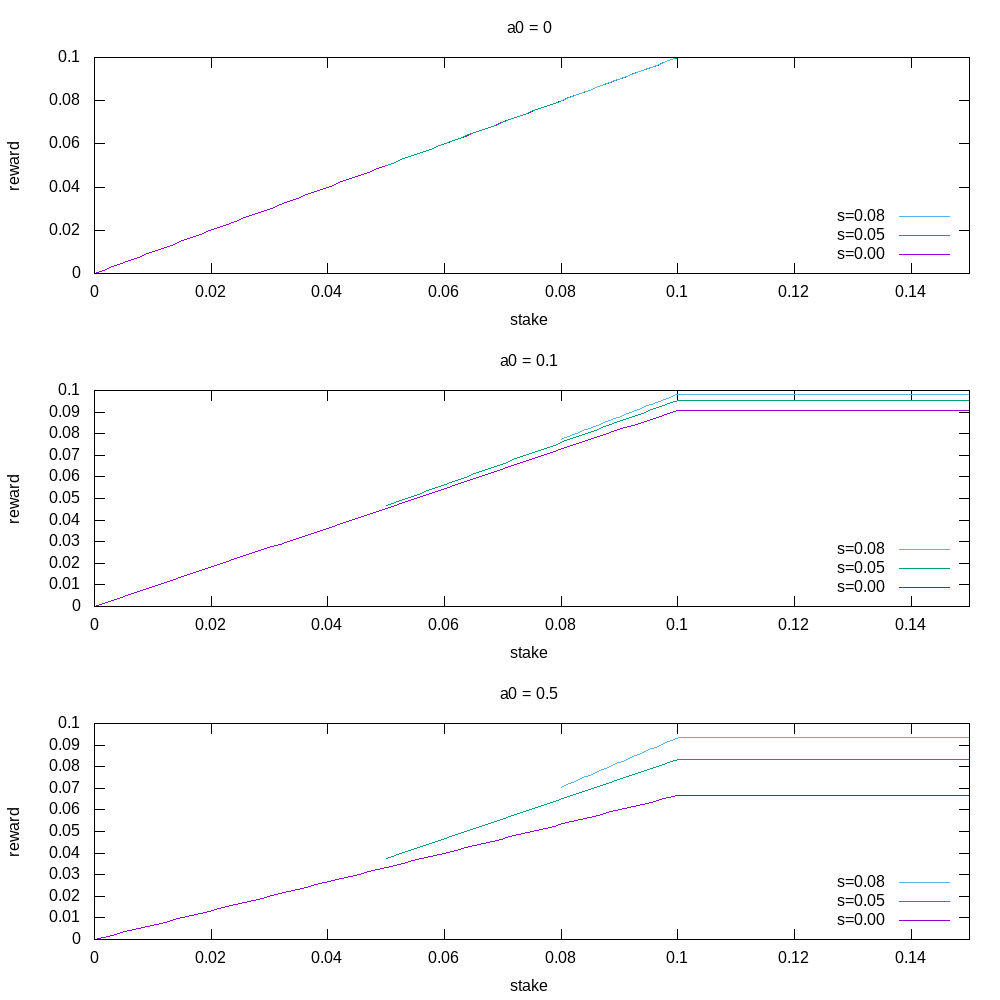
\includegraphics[width=10cm]{rewards.png}
\caption{Effect of different choices for \(a_0\)\label{figrewards}}
\end{figure}

See figure \ref{figrewards} for the effect of various choices for
\(a_0\) on pool rewards (for \(k=10\)).

\subsubsection{\texorpdfstring{\(\rho\)}{\textbackslash{}rho}}\label{rho}

In order to determin the inflation rate per epoch \(\rho\), we need four
more pieces of information:

\begin{itemize}
\item
  The expected \emph{exchange rate} \(e\) from ADA to USD (in USD/ADA).
\item
  The average \emph{costs} \(c\) (in USD) to run a pool for one year.
\item
  The average \emph{transaction fees} \(F\) (in ADA) paid during one
  epoch.
\item
  The expected ratio \(r\) of \emph{rewards} per year per staked ADA.
\end{itemize}

The available rewards for one epoch (assuming an equilibrium state with
\(k\) pools and noticing that there are \(\frac{365}{5}=73\) epochs per
year) will be \[
    \left(1-\tau\right)\cdot\bigl(F + \rho\cdot\left(T\infty - T\right)\bigr) - \frac{k\cdot c}{73\cdot e}.
\] On the other hand, \emph{expected} rewards per epoch are \[
    T\cdot\left(\sqrt[73]{1+r}-1\right).
\] Equating the two, we get \[
    \rho=\frac{T\cdot\left(\sqrt[73]{1+r}-1\right)-(1-\tau)\cdot F+\frac{k\cdot c}{73\cdot e}}{\left(1-\tau\right)\cdot\left(T_\infty-T\right)}.
\] For example, using

\begin{itemize}
\item
  \(k=100\),
\item
  \(T=31,000,000,000\,\mathrm{ADA}\),
\item
  \(T_\infty=45,000,000,000\,\mathrm{ADA}\),
\item
  \(e=0.5\,\mathrm{USD/ADA}\),
\item
  \(c=1,000\,\mathrm{USD}\),
\item
  \(F=2,000\,\mathrm{ADA}\) and
\item
  \(r=0.05\),
\item
  \(\tau=0.2\),
\end{itemize}

we would get \[
    \rho=\frac
        {31,000,000,000\cdot\left(\sqrt[73]{1+0.05}-1\right)-0.8\cdot 2000+\frac{100\cdot 1000}{73\cdot 0.5}}
        {0.8\cdot\left(45,000,000,000 - 31,000,000,000\right)}
    \approx
    0.0019.
\] This would correspond to reducing the remaining amount of available
ADA by \({1.0019}^{73}-1\approx 0.144=14.4\%\) per year (which sounds
awfully high\ldots).

\subsubsection{\texorpdfstring{\(\tau\)}{\textbackslash{}tau}}\label{tau}

Setting \(\tau\) is a policy decision; we will probably use
\(\tau=0.2\), i.e.~20\% of available epoch rewards will be sent to the
treasury.

\subsubsection{\texorpdfstring{\(\gamma\)}{\textbackslash{}gamma}}\label{gamma}

Setting \(\gamma\) is also a policy decision. Having said this, values
of \(\gamma<1\) seem to be preferable, because pool operators
occasionally missing one or two slots will not be punished too harshly.

To help with the task of deciding on a reasonable value for \(\gamma\),
we show the effect of different values on a potential pool that was
elected to create 100 pools in a given epoch. The table below shows the
ratio of rewards paid for varying numbers of missed slots and values of
\(\gamma\):

\begin{tabular}[t]{rrrrr}
    missed slots & $\gamma=1$ & $\gamma=0.7$ & $\gamma=0.5$ & $\gamma=0.3$ \\
    \hline
      0 & 1.0000 & 1.0000 & 1.0000 & 1.0000 \\
      1 & 0.9900 & 0.9930 & 0.9950 & 0.9970 \\
      5 & 0.9500 & 0.9647 & 0.9747 & 0.9847 \\
     10 & 0.9000 & 0.9289 & 0.9487 & 0.9689 \\
     50 & 0.5000 & 0.6156 & 0.7071 & 0.8123 \\
    100 & 0.0000 & 0.0000 & 0.0000 & 0.0000 \\
\end{tabular}

\section{Satisfying the Requirements}\label{satisfying-the-requirements}

In the following, we describe how the requirements listed in
\ref{requirements} are satisfied by the design in this document.

\ref{proof-of-eligibility} Proof of Eligibility

: The leader election process takes delegation via pointer addresses and
heavyweight certificates into account
(\ref{leader-election-block-validity-and-randomness-generation}), so the
leader schedule will contain the key of the party that is expected to
sign the block (either a stake pool operator or an individual
stakeholder).

\begin{verbatim}
If a lightweight certificate is used, it will be posted to the
block header, which will also prove eligibility.
\end{verbatim}

\ref{visibility-of-delegation-on-the-blockchain} Visibility of
Delegation on the Blockchain

: Delegation via heavyweight certificates and pointer addresses is
visible on the blockchain. Delegation via lightweight certificates
should only be used for hot/cold key management. Thus, it is not
relevant for the rewards sharing process, and does not need to be
visible on the chain.

\ref{restricting-chain-delegation} Restricting Chain Delegation

: Chain delegation is properly restricted, as described in
\ref{chain-delegation}.

\ref{cheap-re-delegation} Cheap Re-Delegation

: Re-delegation can be performed cheaply with multi-input transactions.

\ref{neutral-addresses} Neutral Addresses

: The design includes enterprise addresses (\ref{enterprise-address}),
which are disregarded by the PoS protocol.

\ref{sybil-attack-protection-at-stake-pool-level} Sybil Attack
Protection at Stake Pool Level

: Stake pool operators are expected to pledge a deposit to their pools
that has an influence on the rewards that stake pool members will
receive, and on the position of the stakepool in the listing displayed
to stakeholders (\ref{stakepool-registration},
\{display-of-stake-pools-in-the-wallet\}, \todo{add reference
to rewards function once document is merged with incentives doc}).

\begin{verbatim}
Since this pledge cannot be shared between multiple pools,
creating $n$ viable stake pools will require funds linear in $n$.
\end{verbatim}

\ref{address-nonmalleability} Address Nonmalleability

: Protection against the malleability attack is described in
\ref{address-recognition}.

\ref{public-spending-keys-should-not-be-disclosed-prematurely} Public
Spending Keys Should not be Disclosed Prematurely

: The introduction of a dedicated staking key (\ref{address-structure})
avoids the need to use the payment key for delegation purposes.

\ref{mitigate-key-exposure} Mitigate Key Exposure

: Stake pool operators can and should use lightweight certificates for
hot/cold key management, as described in
\ref{lightweight-delegation-certificates}.

\ref{handle-inactive-stake-pools} Handle Inactive Stake Pools

: We have two mechanisms for dealing with inactive stake pools. Stake
pools can be retired via a retirement certificate
(\ref{stake-pool-registration-and-retirement-certificates}. If a stake
pool ceises to operate without being properly retired, its key will be
detected as a stale staking key as described in \ref{stale-stake}.

\ref{avoid-hard-transition} Avoid Hard Transition

: As described in \ref{transition-from-bootstrap-phase}, at the
transition from Byron to Shelley, all stake will initially stay
delegated with the core nodes of the Byron network, avoiding a hard
transition with temporarily undelegated stake.

\ref{change-delegation-without-spending-key} Change Delegation Without
Spending Key

: Delegation of cold wallets is described in
\ref{delegation-of-cold-wallets}, and does not require having the
spending key of the cold wallet online.

\ref{master-recovery-key} Master Recovery Key

: Wallet recovery is described in \ref{wallet-recovery-process}, and
does not require any information in addition to the master key.

\ref{address-recognition} Address Recognition

: Wallets will recognise addresses belonging to it by looking at the
payment key hash part of the address, as described in
\ref{address-recognition-1}.

\ref{wallet-should-be-runnable-on-independent-devices} Wallet should be
Runnable on Independent Devices

: With the caveats listed in that requirement, nothing in this document
requires wallets running on different devices to share state.

\ref{maintain-privacy} Maintain Privacy

: The default delegation mechanism (\ref{basic-delegation}) uses pointer
addresses, so addresses of the same wallet are not connected in an
obvious way.

\ref{short-addresses} Short Addresses

: The goal of having reasonably short addresses has guided the design of
delegation, and we do not see an obvious way of making them even
shorter, while still satisfying the rest of the requirements.

\appendix

\section{Assessment of Rewards Sharing
Mechanisms}\label{assessment-of-rewards-sharing-mechanisms}

\subsection{General Considerations}\label{general-considerations}

\begin{enumerate}
\def\labelenumi{\arabic{enumi}.}
\item
  We use HD Wallets to provide some level of anonymity to stakeholders.
  We would not like to abandon this anonymity for the ability to share
  rewards.

  \begin{itemize}
  \item
    To preserve this level of anonymity HD wallet users will need to
    associate separate staking keys with each HD wallet generated
    address.
  \end{itemize}
\item
  We wish to avoid arbitrary growth in the UTxO (or any other globally
  replicated record, eg contents of epoch boundary blocks).

  \begin{itemize}
  \item
    This is potentially at odds with the rewarding of all stakeholders
    at all epochs
  \end{itemize}
\item
  We want to avoid creating dust (entries in the UTxO that are so small
  that including them in a transaction is not economical, since their
  balance is close to or even less than the increase in fees resulting
  from including another input).

  \begin{itemize}
  \item
    The systemic issue is that dust is likely to have an unbounded
    lifetime in the UTxO
  \item
    Transaction fee structure could be modified to remove the
    transaction cost constraint. The requirement on action by the
    receiver still remains.
  \end{itemize}
\item
  The network has a finite capacity to process transactions. We should
  avoid using a significant fraction of this capacity for sharing
  rewards. In particular, we want to avoid causing unreasonable spikes
  in the transaction rate. Those could either bring the system down on
  their own, or act as an invitation to a timed DoS attack.
\item
  The stake pool operator should not be required to take an action to
  initiate sharing rewards with members.
\item
  Verifying that a reward is legitimate will require a node to access
  some information (like the leader schedule of the epoch in which the
  reward was earned, as well as the delegation pattern at the time the
  leader election for that epoch took place). The time and space
  complexity for this should be constant in the size of the blockchain
  and/or the UTxO of non-reward entries.
\end{enumerate}

Unless we want to give up on anonymity (1.), each address has to
separately receive rewards. Together with 2., 3., and 4., this severely
restricts any approach that distributes rewards using ordinary
transactions.

\subsubsection{Hierarchy of desirability of reward
distribution}\label{hierarchy-of-desirability-of-reward-distribution}

\begin{itemize}
\item
  Reward stakeholders on the basis of their holding at an epoch boundary

  \begin{itemize}
  \item
    Stakeholders are not explicitly represented - there can be a proxy
  \item
    One representation of stake delegation (direct to stake pool) which
    has the property of anonymity-via-aggregation. This, combined with
    the desire to not require stakepools to do the distribution a UTxO
    centric reward distribution mechanism.
  \end{itemize}
\item
  Reward stakeholders that ~maintain a UTxO/stake over the total epoch
  length.

  \begin{itemize}
  \item
    This may be seen a ``regressive'' property in that it would not
    reward those stakeholders who engage in high-velocity value
    movements (e.g make use of the HD wallet).
  \item
    This is a property of certain solutions.
  \end{itemize}
\end{itemize}

\subsubsection{Summary of key points of when rewards are
calculated}\label{summary-of-key-points-of-when-rewards-are-calculated}

\begin{itemize}
\item
  Point in Time

  \begin{itemize}
  \item
    Just considers addresses at an epoch boundary
  \end{itemize}
\item
  Duration in Time

  \begin{itemize}
  \item
    Set of stakeholder address and pool arrangement is fixed at an epoch
    boundary (say epoch \(N-1\) to epoch \(N\))
  \item
    Rewards are calculated at the transition from epoch \(N\) to epoch
    \(N+1\)
  \item
    Only stakeholder addresses that have non-zero associated value at
    the epoch \(N\) to \(N+1\) boundary (i.e have ~value at both the
    epoch \(N-1\) to \(N\) and the epoch \(N\) to \(N+1\) boundaries)
    will be eligible to receive rewards

    \begin{itemize}
    \item
      Noting that this could interact badly with HD wallet users
    \end{itemize}
  \end{itemize}
\end{itemize}

\subsection{Approaches that are Ruled
Out}\label{approaches-that-are-ruled-out}

\subsubsection{Manual Sharing}\label{manual-sharing}

In this approach, only stake pool operators are rewarded directly by the
system, and it is their responsibility to share rewards with members of
the pool.

This approach has been ruled out, since it:

\begin{enumerate}
\def\labelenumi{\arabic{enumi}.}
\item
  requires additional trust in stake pool operators to do this correctly
  (5.)
\item
  requires at least stake pool operators to group the addresses of each
  member, to keep the volume of transactions somewhat reasonable (1.,
  2., 3., and 4.)
\item
  The rewards for members that did not contribute much stake are likely
  to be dust (3.)
\end{enumerate}

\subsubsection{Automatically Issue Transactions Each
Epoch}\label{automatically-issue-transactions-each-epoch}

In this approach, the system automatically distributes rewards at the
end of an epoch, by sending transactions with outputs to every address
that delegated to a stake pool that produced at least one block during
that epoch.

This approach has been ruled out, since it:

\begin{enumerate}
\def\labelenumi{\arabic{enumi}.}
\item
  Leads to a super-linear growth of the UTxO, creating an output per
  address per epoch (2.)
\item
  Is likely to create lots of dust for small stakeholders (3.)
\item
  Will lead to a huge burst of transactions, proportional to the number
  of addresses with non-zero balance in the system (4.). This could be
  lessened somewhat by sending the transactions over the course of the
  following epoch, but it would still use up a large fraction of the
  system's ability to process transactions (4.)
\end{enumerate}

\paragraph{Complexity}\label{complexity}

\begin{itemize}
\item
  Creates one ``UTxO'' per non-zero address at the boundary/duration -
  this would create (today) \textasciitilde{}650k transactions per epoch
\end{itemize}

\subsubsection{Let Members Collect
Rewards}\label{let-members-collect-rewards}

An alternative is to let every stake pool member be responsible for
collecting their own rewards. This approach has the virtue that members
could wait several epochs until they had accumulated enough rewards to
warrant a transaction. The overall rate of transactions for sharing
rewards would be reduced, the transactions would not come in bursts, and
the problem of creating dust could be avoided.

However, this approach has been ruled out, since it:

\begin{enumerate}
\def\labelenumi{\arabic{enumi}.}
\item
  Requires nodes to cache or quickly retrieve the whole history of
  leader schedules, as well as the delegation configurations at the time
  of each leader selection (6.)
\end{enumerate}

\subsection{Feasible Approaches}\label{feasible-approaches}

\subsubsection{Automatic UTxO Updates}\label{automatic-utxo-updates}

This unique approach circumvents the problems of transaction rates, dust
entries, and UTxO growth, at the expense of introducing an implicit
modification of the UTxO set.

After an epoch, each UTxO entry that delegated to a stake pool will have
its balance updated to reflect the rewards that it earned. Since the
update can be derived from information that every node has (leader
schedule and delegation pattern at the last election), it can be carried
out by each node individually.

Sadly, this approach does come with its own drawbacks:

\begin{enumerate}
\def\labelenumi{\arabic{enumi}.}
\item
  It is not yet clear how a lightweight wallet would determine the
  correct UTxO set.
\item
  It introduces an implicit update of each UTxO entry, a huge moving
  part that makes it much harder to reason about the system.
\item
  Transactions that are formed before an update, but included after it,
  will have a larger total input than the issuer anticipated.
\item
  (Public Perception) This may be perceived as subverting the notion of
  immutability of the blockchain (at least in its UTxO model)
\end{enumerate}

\subsubsection{Lotteries per Stakepool}\label{lotteries-per-stakepool}

A variation of ``Automatically Issue Transactions Each Epoch'', this
approach avoids dust and creating a huge number of transactions by
performing one lottery per stake pool. A number of winning addresses is
determined, and the rewards are distributed amongst those addresses. The
probability of any address winning the lottery is proportional to the
stake that that address contributed to the pool. Benefits of this
approach are:

\begin{enumerate}
\def\labelenumi{\arabic{enumi}.}
\item
  The number of transactions will be proportional to the number of stake
  pools that signed at least one block, which is nicely bounded by the
  number of slots in an epoch.
\item
  The chances of creating dust entries is fairly low, since each winning
  address will receive a sizeable fraction of the pools rewards.
\item
  There is no need to group addresses per stake pool member.
\item
  Possibly -- this would have to be investigated by legal -- this could
  make Ada less like a security.
\end{enumerate}

The remaining drawbacks are:

\begin{enumerate}
\def\labelenumi{\arabic{enumi}.}
\item
  It will still create a burst of transactions. This could be prevented
  by staggering the transactions that share rewards
\item
  An individual stake pool member will on average receive the same
  rewards as with any of the other approaches, but it will be much less
  predictable. This might be problematic from a Public Perception
  perspective.
\item
  (Public Perception) although (in the limit) this is the same outcome
  as sharing, apparently most humans don't see things that way - see
  Prospect Theory (https://en.wikipedia.org/wiki/Prospect\_theory) -
  they would prefer known outputs (even if smaller) than unknown ones.
  ~An additional indicator of human response might be to look at a
  similar mechanism (random rewards for depositing a fixed stake) has
  run since 1956. ~Premium Bonds
  (https://en.wikipedia.org/wiki/Premium\_Bond) - computer nerds /
  crypto nuts should note who helped create the original ERNIE). The
  public might like the gambling aspect, businesses might not!
\end{enumerate}

\subsubsection{Reward accounts per stake
key}\label{reward-accounts-per-stake-key}

This is in some sense a variation of the ``Automatic UTxO updates'', but
trying to address its shortcomings.

Add a new class of address, reward addresses, based on a stake key.
These addresses have special rules:

\begin{itemize}
\item
  Account style accumulation, not UTxO style
\item
  Paid into only by reward payout mechanism, never by normal Txs.
\item
  Withdrawn from by normal Txs, using the stake key as the witness.
\end{itemize}

At the end of an epoch once the pool rewards are known, identify all the
stake keys that contribute to a pool and the rewards per stake key. The
system implicitly issues a transaction/state-change to pay out rewards
to each stake key reward account. These rewards accumulate if they are
not withdrawn.

It is to be decided if value held in a reward account contributes to
stake that is delegated to a stake pool and hence itself attracts
rewards. Doing so would reduce the incentive to withdraw early and would
mean the stake corresponding to the reward is not effectively offline.
It should be possible to do so since the value in the reward account is
identified with the stake key, and the delegation of the stake key is
known.

Withdrawal of rewards is done similarly to the withdrawal transaction
from the Chimeric Ledgers paper. This uses the stake key as the witness,
which reveals the public part of the stake key. Note that this also
requires a nonce to prevent replay attacks. One simplifying approach
here might be to use the epoch number as the nonce, and to require the
whole reward be withdrawn, and hence this could only be valid once
within the epoch.

This aggregation of rewards -- account style -- is the key to resolving
the UTxO storage asymptotic complexity problem. It is the same
fundamental approach as the ``Automatic UTxO updates'' approach, but
putting the aggregation off to into a separate class of addresses, so
that normal addresses remain in a pure UTxO style.

The asymptotic storage complexity of the ledger state (i.e.~UTxO size)
is linear in the number of stake keys, but is unrelated to the number of
epochs that have passed. This is in contrast to approaches that create
UTxO entries for rewards on every epoch.

An important constraint for this approach is that is relies on stake
keys belonging to stakeholders. This means every stakeholder address
must be associated with some stake key belonging to the stakeholder.
This means it is not possible to use addresses that point directly to a
stakepool and still be able to have a corresponding reward address,
since there is not stake key to use for that reward address. There are
alternatives to using addresses that point directly to pools, but these
either reduce privacy or increase fees. One alternative that reduces
privacy is for all addresses in a wallet to share the same stake key
(either as base addresses, or a base address and pointer addresses to
that stake key). This reduces privacy since all addresses in the wallet
can be tied together by using the same stake key. Another alternative is
to use a separate stake key for every address. This means using one
delegation certificate per address. This increases the fees for creating
addresses in a wallet following this policy, and for changing delegation
choices. In principle there's a sliding scale between the two previous
option , using a number of stake keys, more than one but fewer than the
number of addresses.

\begin{itemize}
\item
  stake in reward accounts is ordinary stake, and hence is counted in
  delegation to stake pools, or can be used directly in creating blocks.
\item
  There is a potential interaction with UTxO deposit/refund approach. It
  may be that (because the refund is smaller than the reward) that
  negative values need to be stored. Though this may be able to done by
  some registration cost.
\end{itemize}

Advantages:

\begin{itemize}
\item
  doesn't ``mutate'' the UTxO. This reduces conceptual and
  implementation complexity. It does not disrupt wallets and other
  things based on the UTxO model.
\end{itemize}

Disadvantages:

\begin{itemize}
\item
  introduces limited degree of account style chimeric ledgers. This adds
  a degree of conceptual and implementation complexity.
\item
  Cannot use pointer addresses directly to stake pools. Increases fee
  and complexity cost of maintaining wallet privacy.
\item
  Unless people stick to a single staking key (which would immediately
  mean they give up all privacy, not a choice most people would be
  comfortable with I suspect), we basically end up creating lots of
  staking keys, to which we would only deposit once, and withdraw from
  once -- in other words, we'd have reinvented UTxO entries, and the
  accumulation does not help.
\end{itemize}

\section{Draft formal specification for delegation}
\label{formal-specification-for-delegation}

This appendix is intended to be the start of a formal specification of the
ledger rules for Cardano, with a focus on the rules for delegation in the
Cardano Shelly release. The purpose is to help clarify the design and to give
a reasonable starting point for tests and an implementation.

\newcommand{\powerset}[1]{\mathbb{P}(#1)}
\newcommand{\restrictdom}{\lhd}
\newcommand{\subtractdom}{\mathbin{\slashed{\restrictdom}}}
\newcommand{\restrictrange}{\rhd}

\begin{figure}[h]

\emph{Primitive types}
%
\begin{equation*}
\begin{array}{r@{~\in~}lr}
  txid
& \mathsf{TxId}
& \text{transaction id}
\\
  ix
& \mathsf{Ix}
& \text{index}
\\
  addr
& \mathsf{Addr}
& \text{address}
\\
  c
& \mathsf{Coin}
& \text{currency value}
\end{array}
\end{equation*}
%
\emph{Derived types}
%
\begin{equation*}
\begin{array}{r@{~\in~}l@{\qquad=\qquad}r@{~\in~}lr}
  tx
& \mathsf{Tx}
& (inputs, outputs)
& \powerset{\mathsf{TxIn}} \times (\mathsf{Ix} \mapsto \mathsf{TxOut})
& \text{transaction}
\\
  txin
& \mathsf{TxIn}
& (txid, ix)
& \mathsf{TxId} \times \mathsf{Ix}
& \text{transaction input}
\\
  txout
& \mathsf{TxOut}
& (addr, c)
& \mathsf{Addr} \times \mathsf{Coin}
& \text{transaction output}
\\
  utxo
& \mathsf{UTxO}
& txin \mapsto txout
& \mathsf{TxIn} \mapsto \mathsf{TxOut}
& \text{unspent tx outputs}
\end{array}
\end{equation*}
%
\emph{Functions}
%
\begin{equation*}
\begin{array}{lr}
  \mathsf{txid} \in \mathsf{Tx} \to \mathsf{TxId}
& \text{compute transaction id}
\end{array}
\end{equation*}

\caption{\label{fig:basic_definitions}Basic Definitions}
\end{figure}


\begin{figure}

\begin{align*}
& \mathsf{txins} \in \mathsf{Tx} \to \powerset{\mathsf{TxIn}}
& \text{transaction inputs} \\
& \mathsf{txins} ~ (\mathit{inputs}, \,\underline{\phantom{a}}\,) = \mathit{inputs}
\\[1em]
& \mathsf{txouts} \in \mathsf{Tx} \to \mathsf{UTxO}
& \text{transaction outputs as UTxO} \\
& \mathsf{txouts} ~ \mathit{tx} =
  \left\{ (\mathsf{txid} ~ \mathit{tx}, \mathit{ix}) \mapsto \mathit{txout} ~
  \middle| \begin{array}{l@{~}c@{~}l}
             (\,\underline{\phantom{a}}\,,\, \mathit{outputs}) & = & \mathit{tx} \\
             \mathit{ix} \mapsto \mathit{txout} & \in & \mathit{outputs}
           \end{array}
  \right\}
\\[1em]
& \mathsf{balance} \in \mathsf{UTxO} \to \mathsf{Coin}
& \text{UTxO balance} \\
& \mathsf{balance} ~ utxo = \sum_{(\,\underline{\phantom{a}}\, ~ \mapsto (\,\underline{\phantom{a}}\,, \,c)) \in \mathit{utxo}} c
\end{align*}

\begin{align*}
  \mathit{ins} \restrictdom \mathit{utxo}
& = \{ i \mapsto o \mid i \mapsto o \in \mathit{utxo}, ~ i \in \mathit{ins} \}
& \text{domain restriction}
\\
  \mathit{ins} \subtractdom \mathit{utxo}
& = \{ i \mapsto o \mid i \mapsto o \in \mathit{utxo}, ~ i \notin \mathit{ins} \}
& \text{domain exclusion}
\\
  \mathit{utxo} \restrictrange \mathit{outs}
& = \{ i \mapsto o \mid i \mapsto o \in \mathit{utxo}, ~ o \in \mathit{outs} \}
& \text{range restriction}
\end{align*}

\caption{\label{fig:auxiliary_ops}Transaction and UTxO operations}
\end{figure}


\begin{figure}

\emph{Key types}
%
\begin{equation*}
\begin{array}{r@{~\in~}lr}
  sk
& \mathsf{SKey}
& \text{signing key}
\\
  vk
& \mathsf{VKey}
& \text{verification key}
\\
  hk
& \mathsf{Hash}
& \text{hash of a key}
\end{array}
\end{equation*}
%
\emph{Functions and relations}
%
\begin{equation*}
\begin{array}{r@{~\in~}lr}
  \mathsf{hash} & \mathsf{VKey} \to \mathsf{Hash}
& \text{hashing a key}
\\
  \mathsf{sign} & \mathsf{SKey} \times \mathsf{Data} \to \mathsf{Sig}
& \text{signature}
\\
  \mathsf{verify} & \mathsf{VKey} \times \mathsf{Data} \times \mathsf{Sig}
& \text{verification}
\end{array}
\end{equation*}
%
\emph{Verification property}
%
\begin{align*}
\forall ~ \text{key pairs} & ~ (sk, vk), m \in \mathsf{Data}, \sigma \in \mathsf{Sig}. \\
     & \mathsf{verify} (\mathit{vk}, m, \sigma) \\
\iff & \\
     & \mathsf{sign} (\mathit{sk}, m) = \sigma
\end{align*}
%
\emph{Notation for serialised, signed and verified data}
%
\begin{equation*}
\begin{array}{lcl}
  \llbracket x \rrbracket
& \text{is}
& \text{the serialised representation of } x
\\[0.2em]
  \llbracket x \rrbracket_\sigma
& \iff
& \exists \mathit{sk}. ~ \mathsf{sign} (sk, \llbracket x \rrbracket) = \sigma
\\[0.2em]
  \mathcal{V}_{\mathit{vk}}\llbracket x \rrbracket_\sigma
& \iff
& \mathsf{verify} (\mathit{vk}, \llbracket x \rrbracket, \sigma)
\end{array}
\end{equation*}

\caption{\label{fig:crypto}Cryptographic operations for signing and verifying}
\end{figure}

\begin{figure}


\begin{equation*}
\frac{
}{
\mathcal{G}_{\mathsf{utxo}}, \emptyset
}
\textsc{genesis}
\end{equation*}

\begin{equation*}
\frac{
\mathsf{txins} ~ \mathit{tx} \subseteq \mathit{utxo} \quad \mathsf{balance}~(\mathsf{txouts}~\mathit{tx}) \leq \mathsf{balance}~(\mathsf{txins} ~ \mathit{tx} \restrictdom \mathit{utxo})
}{
\mathit{utxo}, \Lambda \xlongrightarrow[\textsc{transaction}]{\mathit{tx}} (\mathsf{txins} ~ \mathit{tx} \subtractdom \mathit{utxo}) \cup \mathsf{txouts}~\mathit{tx},  \Lambda ; \mathit{tx}
}
\end{equation*}

\caption{\label{fig:transaction_transitions}State transitions for transactions}
\end{figure}


\begin{figure}

\begin{equation*}
\frac{
  \mathit{vk_{sk}} \notin \mathit{stkeys} \quad
  \mathcal{V}_{\mathit{vk_{sk}}}\llbracket\mathit{vk_{sk}}\rrbracket_\sigma
}{
  \mathit{stkeys}, ~ \mathit{accounts}
  \xlongrightarrow[\textsc{register stake key}]{\llbracket\mathit{vk_{sk}}\rrbracket_\sigma}
  \mathit{stkeys} \cup \{\mathit{vk_{sk}}\}, ~
  \mathit{accounts} \cup \{\mathsf{stAcc}~\mathit{vk_{sk}} \mapsto 0\}
}
\end{equation*}

\begin{equation*}
\frac{
  \mathit{vk_{sk}} \in \mathit{stkeys} \quad
  \mathcal{V}_{\mathit{vk_{sk}}}\llbracket\mathit{vk_{sk}}\rrbracket_\sigma
}{
  \mathit{stkeys}, ~ \mathit{accounts}
  \xlongrightarrow[\textsc{deregister stake key}]{\llbracket\mathit{vk_{sk}}\rrbracket_\sigma}
  \mathit{stkeys} \setminus \{\mathit{vk_{sk}}\},
  \{\mathsf{skAcc}~\mathit{vk_{sk}}\} \subtractdom \mathit{accounts}
}
\end{equation*}
%
\\[1em]
%
\begin{equation*}
\frac{
  \begin{array}{c}
  \mathit{cert} = (\mathit{vk_{sp}}, \mathit{owners}, (c, m), \mathit{alt}) \quad\quad \mathsf{hash} ~ \mathit{vk_{sp}} \notin \dom \mathit{stpools} \\
  \mathcal{V}_{\mathit{vk_{sp}}}\llbracket\mathit{cert}\rrbracket_\sigma \quad\quad  \forall \mathit{vk_{sk}} \in \mathit{owners}. ~ \exists \sigma \in \Sigma. ~ \llbracket\mathcal{V}_{\mathit{vk_{sk}}}\mathit{cert}\rrbracket_\sigma
  \end{array}
}{
  \mathit{stpools}, ~ \mathit{accounts}
  \xlongrightarrow[\textsc{register stake pool}]{\llbracket \mathit{cert} \rrbracket_{\sigma,\Sigma}}
  \mathit{stkeys} \setminus \{\mathit{sk}\},
  \{\mathsf{skAcc}~\mathit{sk}\} \subtractdom \mathit{accounts}
}
\end{equation*}

\caption{\label{fig:delegation_transitions}State transitions for delegation}
\end{figure}

\addcontentsline{toc}{section}{References}
\bibliographystyle{apalike}
\bibliography{references}

\end{document}
